\documentclass{scrartcl}
\usepackage[utf8]{inputenc} 
\usepackage[T1]{fontenc}
\usepackage{lmodern}
\usepackage[ngerman]{babel}
\usepackage{courier}
\usepackage{amsmath}
\usepackage{graphicx}
\usepackage{multicol}
\usepackage{geometry}
\usepackage{authblk}
\usepackage[font=scriptsize, labelfont=bf]{caption}
\usepackage{listings}
\usepackage{hyperref}
\usepackage{color}
\usepackage{amssymb}
\usepackage{graphicx}
\usepackage{sidecap}
\newenvironment{Figure}
  {\par\medskip\noindent\minipage{\linewidth}}
  {\endminipage\par\medskip}
  
\usepackage[style=numeric]{biblatex}
\usepackage[babel,german=guillemets]{csquotes}
\usepackage[toc,page]{appendix}
\bibliography{literatur}
  
\definecolor{dkgreen}{rgb}{0,0.6,0}
\definecolor{gray}{rgb}{0.5,0.5,0.5}
\definecolor{mauve}{rgb}{0.58,0,0.82}

\lstset{frame=tb,
  language=C,
  aboveskip=3mm,
  belowskip=3mm,
  showstringspaces=false,
  columns=flexible,
  basicstyle={\small\ttfamily},
  numbers=none,
  numberstyle=\tiny\color{gray},
  keywordstyle=\color{blue},
  commentstyle=\color{dkgreen},
  stringstyle=\color{mauve},
  breaklines=true,
  breakatwhitespace=true,
  tabsize=3
  }


% for skript letters like H...
\usepackage{mathrsfs}

\geometry{verbose,a4paper,tmargin=25mm,bmargin=25mm,lmargin=15mm,rmargin=20mm}

\title{Protokoll zum Versuch Nichtlineare Dynamik und Chaos}
\author{Nicolas Heimann, Jesse Hinrichsen}
\affil{\textit{Universität Hamburg}}
\date{2015}
\begin{document}
\maketitle
\begin{center}
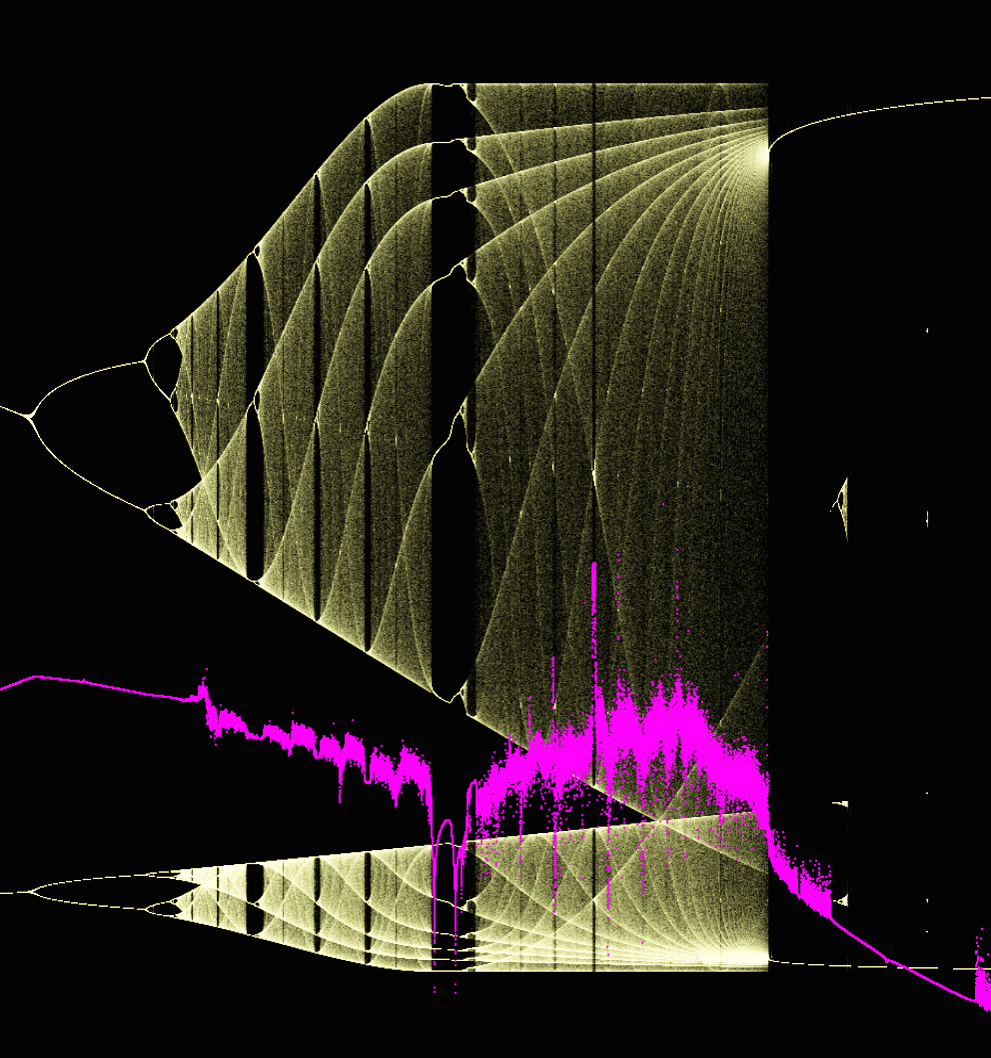
\includegraphics[scale=0.25]{funfunfun} 
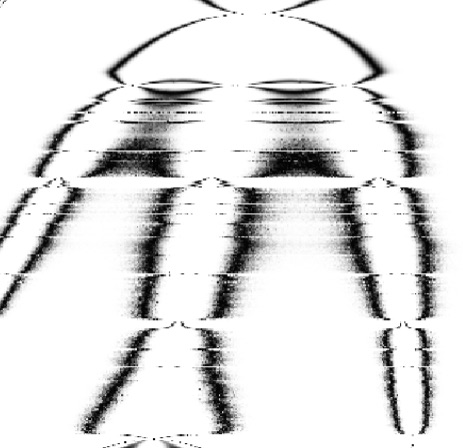
\includegraphics[scale=0.25]{alien} 
\end{center}

\begin{description}
\item ABSTRACT TEXT TODO - vorläufig stand 300815
\end{description}

\section{Einleitung}
In diesem Protokoll haben wir die Eigenschaften von chaotischen System anhand der logistischen Gleichung, der Sinusabbildung, der Duffing-Gleichung und dem LDR Schwingkreis numerisch bestimmt und analysiert. Ebenfalls haben wir den LDR Schwingkreis in einem Experiment anhand eines analogen Oszilloskopes Untersucht.
Alle Plots und Simulationen in diesem Protokoll haben wir im Rahmen des Versuches selber implementiert. Dafür wählten wir als Programmiersprache Python2.7 und nutzten OpenGL4.1 und OpenCL für Visualisierungen und Berechnungen. Der Quellcode ist über github einsehbar: \url{https://github.com/keksnicoh/gl_plotting_experimental}. Bei Abbildungen ist ein entsprechender Quellcodeverweis angegeben. 

Im folgenden bezeichnet $f^2(x) = f(f(x))$

\tableofcontents

\section{Logistische Abbildung}
Die logistische Abbildung ist gegeben durch $f(x_n)=x_{n+1}=rx_n(1-x_n)$. Es zeigt sich das diese einfache Funktionsvorschrift 
bereits chaotisches Verhalten an den Tag legt welches wir im folgenden Abschnitt genauer untersucht haben. Zunächst haben 
wir ein Bifurkationsdiagramm der logistischen Abbildung erzeugt indem wir den Parameter r gegen Iterationspunkte aufgetragen haben. Dabei fixierten wir jeweils ein r und erzeugten eine Folge $x_0 ... x_{1000}$ von welcher wir $x_{500} ... x_{1000}$ gegen die Ordinate aufgetragen haben (Abbildung \ref{fig:bifurkation-sin-nice}).
Das Bifurkationsdiagramm lässt sich in mehrere Bereiche unterteilen. Bis $r=3$ laufen die $x_{500}...x_{1000}$ auf den gleichen Fixpunkt zu. An $r=3$ gabelt sich das Diagramm in zwei Äste auf (Periodenverdoppelung). An $r=3.449$ gibt es eine weitere Perdionenverdopplung und es ist eine Selbstähnlichkeit mit dem Bereich um $r=3$ zu erkennen (fraktale Strukturen). Ab $r=3.569$ entsteht ein chaotischer Bereich in welchem sich aber noch Strukturen feststellen lassen (Bögen, Punkte auf Geraden, freie Bereiche).
\begin{figure}[!htbp]
	\centering
	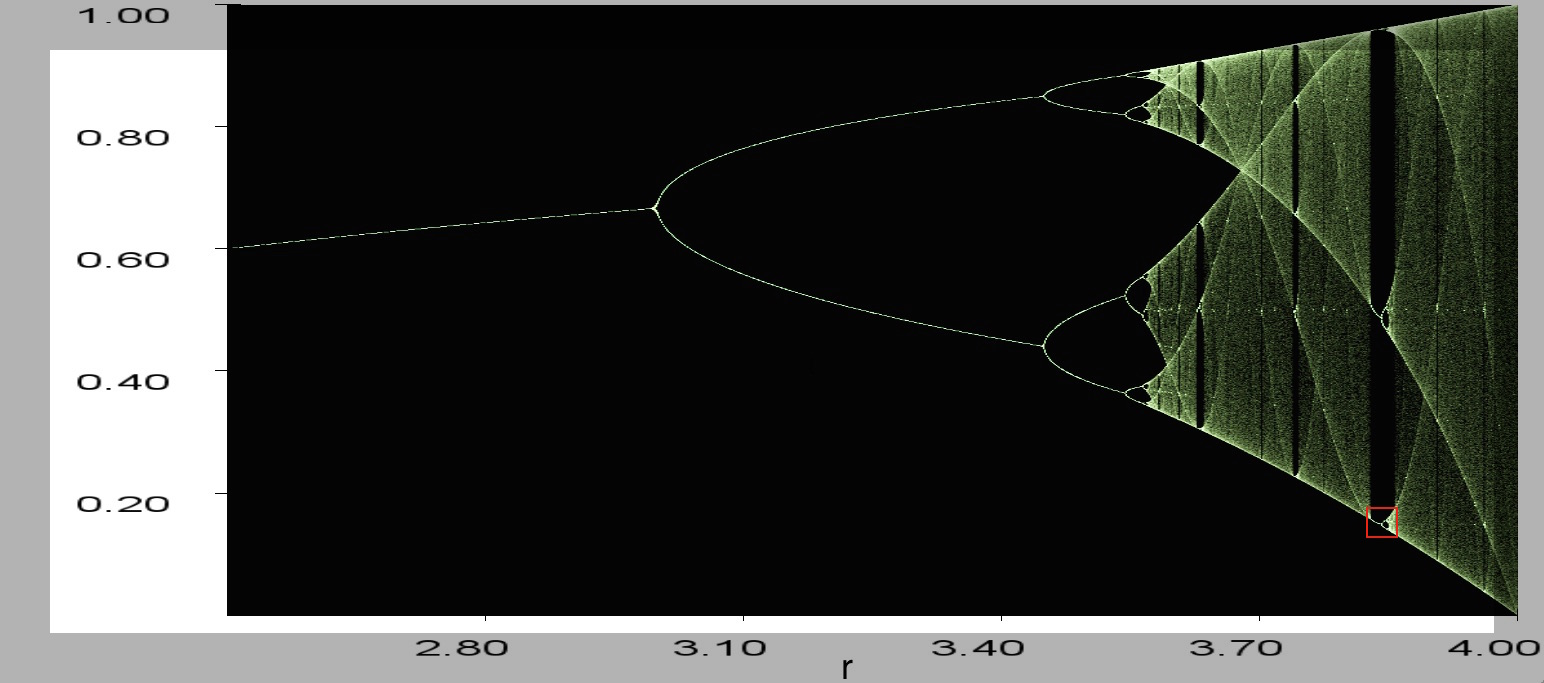
\includegraphics[scale=0.30]{bifurkation}
	\caption{Bifurkationsdiagramm der logistischen Abbildung im Bereich $r\in[2.6,4]$. sourcecode: prak/birukation-logistisch-no-opt.py}
	\label{fig:bifurkation-sin-nice}
\end{figure}
\subsection{Fixpunkte / Stabilitätsbedigung}
Bildet die Funktion einen Punkt idempotent ab, so handelt es sich um einen Fixpunkt, es gilt: $f^n(x)=x$ $\forall n \iff x$ ist Fixpunkt. 
Stabilitätsbedingung:
\begin{equation} |f'(x)|<1 \iff Fixpunkt-stabil \end{equation}
\begin{equation} |f'(x)|>1 \iff Fixpunkt-instabil \end{equation}
Mit $ f(x)=rx(1-x)=x $ folgen die Fixpunkte $x_{0}=0$ und $x_{1}=1-\frac{1}{r}$. Mit der Stabilitätsbedingung (wir betrachten $f'(x)=r-2rx$) folgt für $x_{0}$:
$$-1 < r < 1: x_{0} \text{ stabil}$$
$$r > 1: x_{0} \text{ instabil}$$
Für $x_{1}=1-\frac{1}{r}$ folgt:
$$1 < r < 3: x_1 \text{ stabil}$$
$$r<1 \wedge  r> 3: x_1 \text{ instabil}$$
Abbildung \ref{fig:log-iteration-behavior} zeigt wie sich die Iteration bei unterschiedlichen Parametern verhalten. Für $r>3$ ist $x_1$ nicht mehr stabil. So lässt sich die Aufspaltung im Bifurkationsdiagramm (Abbildung \ref{fig:bifurkation-sin-nice}) für $r>3$ verstehen. Ebenfalls wurde das Konvergenzverhalten der logisitschen Abbildung gegen $x_1$ geprüft indem von den letzten beiden Werten jeweils der Mittelwert gebildet wurde. Bereits nach 30 Iterationen konnten alle $x_1$ für $1 < r \leq 3$ numerisch bestimmt werden. Ab $r>3$ funktioniert diese Methode nicht mehr, da die beiden Äste im Bifurkationsdiagramm nicht Punktsymmetrisch an $x_1$ spiegeln (Abbildung \ref{fig:log-intermittenz-cycles}). In Abbildung \ref{fig:log-iteration-behavior} ist für den Fall $r=3.113$ ebenfalls zu sehen, dass das Konvergenzverhalten asymmetrisch im Vergleich zum Fall $r=2.878$ ist .
Im folgenden untersuchen wir den Zweierzyklus $f^2(x)$.
\begin{equation}x_{n+1}=f_r(x_n)=rx_n(1-x_n)
\Rightarrow x_{n+2}=r^2x_n(1-x_n)(1-rx_n(1-x_n))\end{equation}
\newline
Fixpunktgleichung (Zweierzyklus):
\begin{equation}
x=r^2x(1-x)(1-rx(1-x))
\Rightarrow 
x_{3,4}=\pm\frac{\sqrt{r^2-2 r-3}+r+1}{2 r}
\end{equation}
Da $x_{3,4} \in \mathbb{R} $,  muss $r^2-2 r-3 \geq 0$
\begin{equation}
\Rightarrow r \leq -1 \land r \geq 3
\end{equation}
Für diesen Bereich gibt es folglich 2 weitere Fixpunkte $x_{3,4}$. 
Es gilt:
\begin{equation}
\frac{d}{dx}f^2(x)=-r^2(2x-1)(2r(x-1)x+1)
\end{equation}
Lösungen der Gleichung $|\frac{d}{dx}f^2(x_{3,4})|=1$ sind: $r_0=-1$, $r_1=3$, $r_2=1-\sqrt{6}\approx-1.45$, $r_3=1+\sqrt{6}\approx3.45$. Da die Fixpunkte $x_{3,4}$ nur für $r>3$ und $r<-1$ existieren folgt.
\begin{equation}1-\sqrt{6}< r \leq -1 \wedge 3 \geq r > 1+\sqrt{6}: x_{3,4} \text{ stabil}
\end{equation}
\begin{equation}r < 1-\sqrt{6} \wedge r>1+\sqrt{6}: x_{3,4} \text{ instabil}
\end{equation}

Die logistische Funktion zeigte bei einigen Parametern r Intermittenz (Abbildung \ref{fig:log-intermittenz-cycles}). Intermittenz ist ein Grund für die Verdichtungen welche im choatischen Bereich des Bifurkationsdiagrammes zu sehen sind.

\begin{figure}[!htbp]
\centering
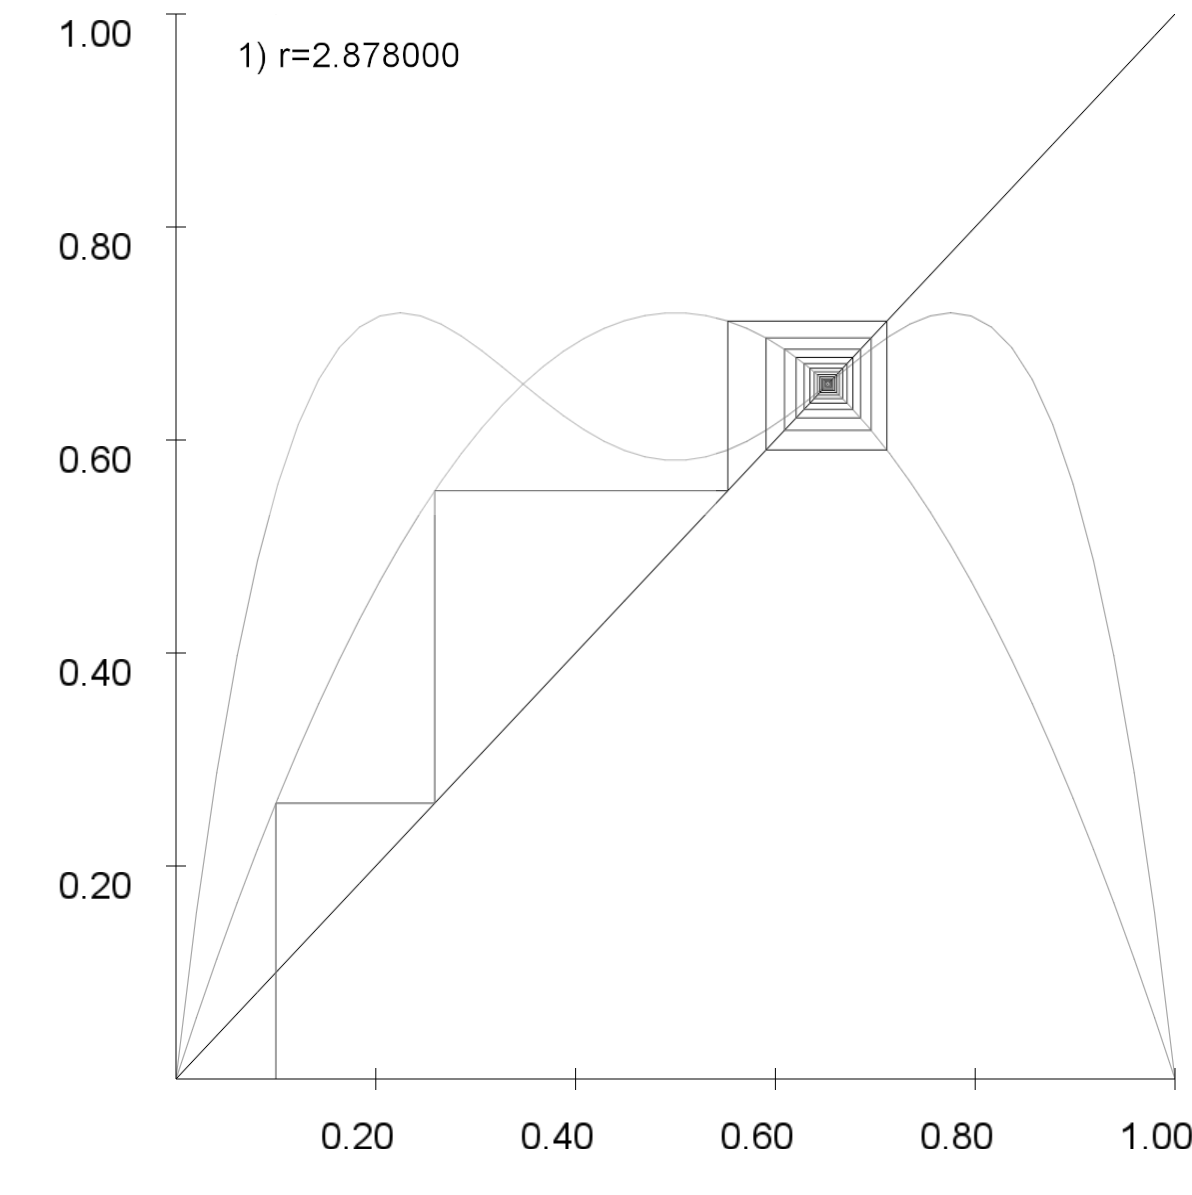
\includegraphics[height=150px]{fixpunkt-2878}
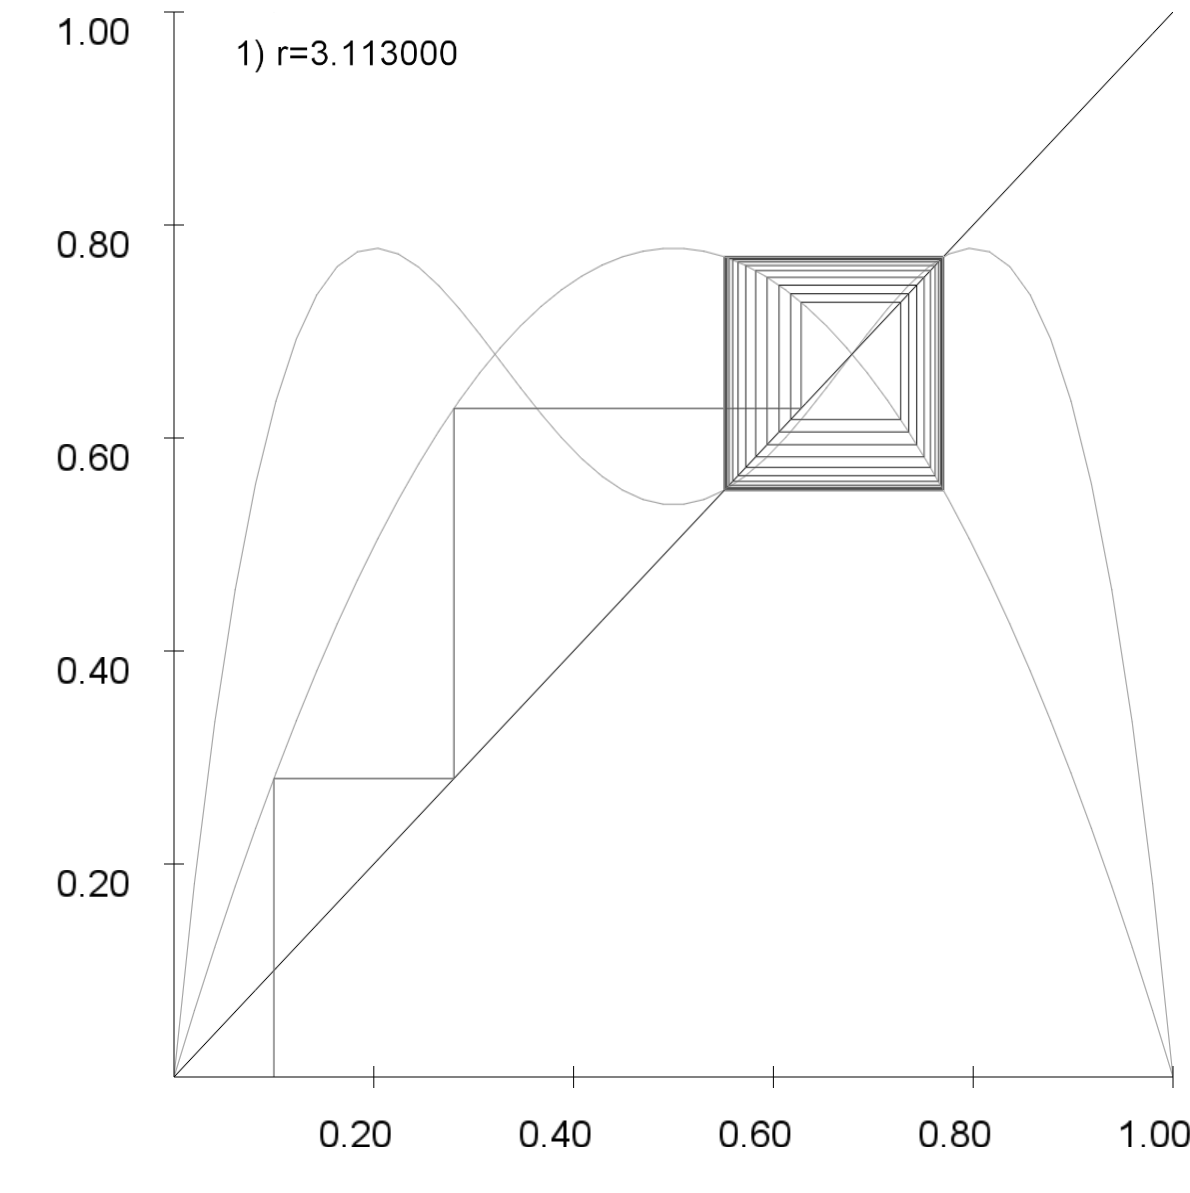
\includegraphics[height=150px]{fixpunkt-311}
\caption{Verlauf der Iterationen bei festem Parameter r. Links: Konvergiert gegen Fixpunkt $x_1$ bei r=2.878. Rechts: Bei r=3.113 ist $x_1$ kein stabiler Fixpunkt mehr. Der Verlauf der logistischen Funktion $f(x)$, $f^2(x)$ sowie die Einheitsgerade $y=x$ sind aufgetragen . Als Linie Verbunden geplottet sind die Folgen ($x_n, 0.0), (x_n, x_{n+1}), (x_{n+1}, x_{n+1}), (x_{n+1}, x_{n+2}), (x_{n+2}, x_{n+2}), (x_{n+2}, x_{n+3}), ...$ Sourcecode: prak/logisitsch-no-opt-behavior.py}. 
\label{fig:log-iteration-behavior}
\end{figure}

\begin{figure}[!htbp]
\centering
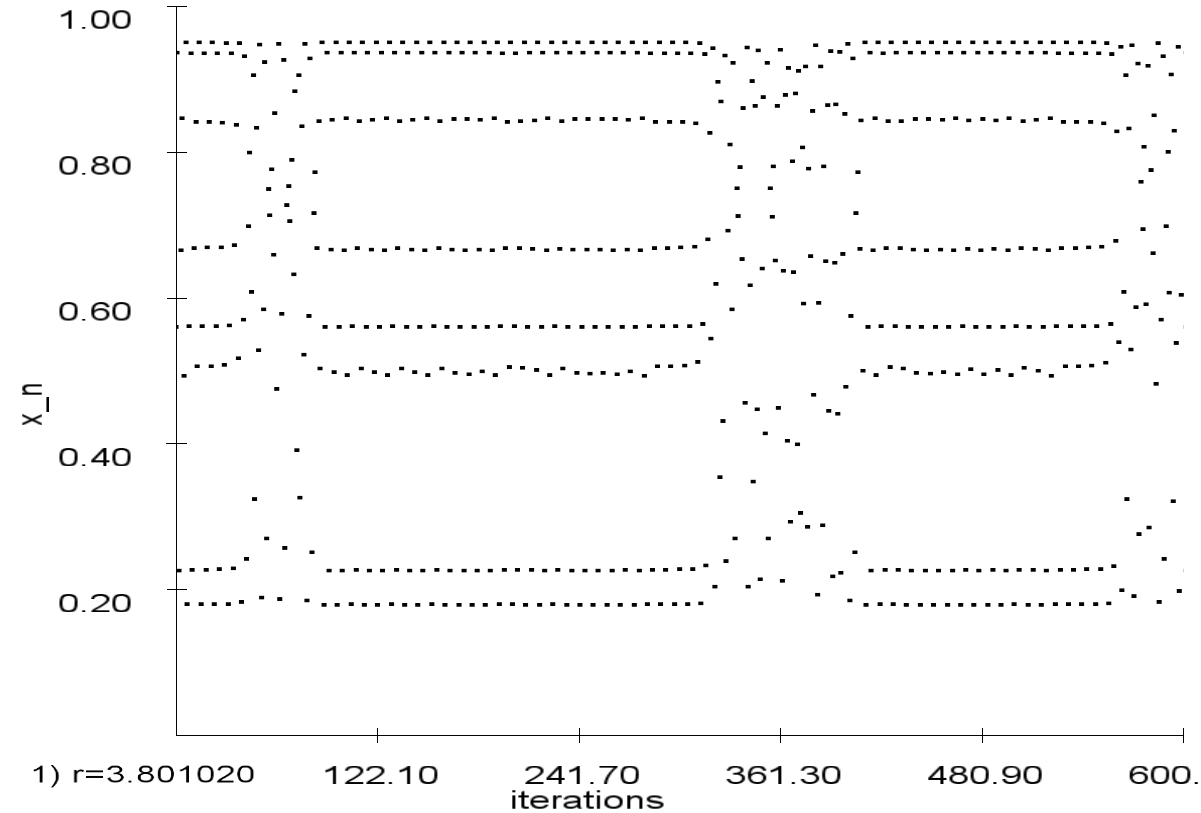
\includegraphics[scale=0.22]{intermittenz}
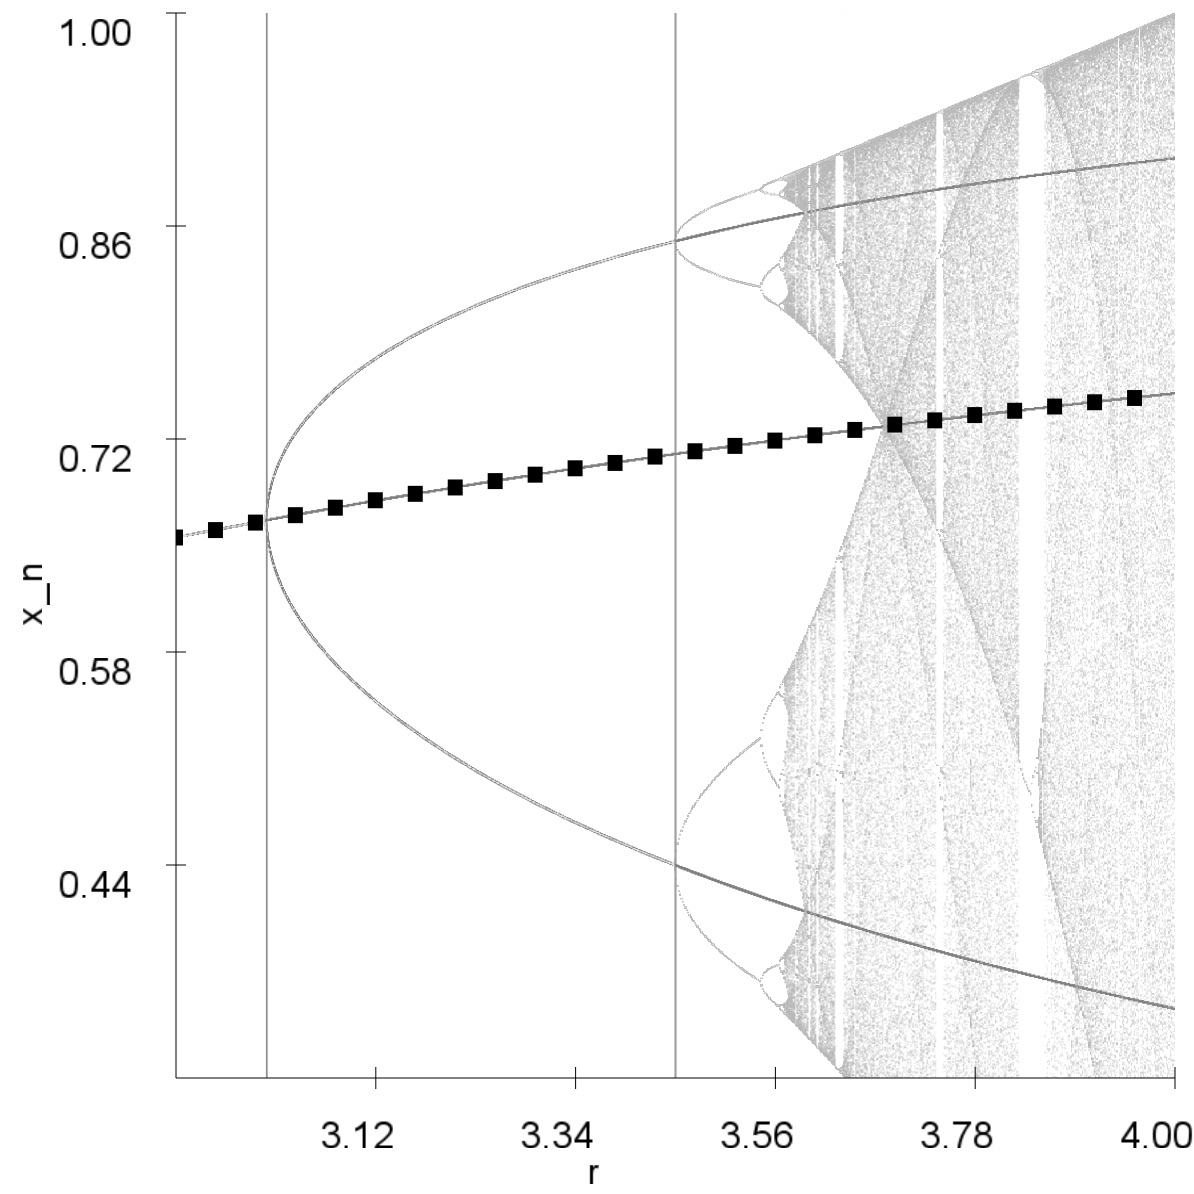
\includegraphics[scale=0.15]{analy-periodenv}
\caption{Logistische Funktion. Links: Intermittenz bei $r=3.80102$. Rechts: Die stabile Lösung des Einerzyklus $x^*$ und die beiden Lösungen des Zweierzyklus $x_{3,4}$. Im Hintergrund das Bifurkationsdiagramm. Die Punkte sind die das Ergebniss der numerischen Berechnung der Fixpunkte $x_1$. Die vertikalen Linien sind an $r=3.0$ und $r=3.44$ und markieren die Stellen wo $|f'(x)|=1$, $|\frac{d}{dx}f^2(x)|=1$ sind. Sourcecode: prak/intermittenz.py, prak/logis-zyklen.py}. 
\label{fig:log-intermittenz-cycles}
\end{figure}

\subsection{Bifurkationspunkt}
Im weiteren betrachten wir das Konvergenzverhalten der logistischen Abbildung bei $r=3$ und Umgebung. Für r<3 kennen wir bereits den Fixpunkt $x_1=1-\frac{1}{r}$. 
Abbildung \ref{fig:log-konv1} (links) trägt den x Wert gegen die Anzahl der Iterationen bei $r=3$ auf. Dabei sei zunächst angemerkt, dass wir bei der Berechnung über einen OpenCL Kernel mit double precision, also float64 anscheinend sehr schnell auf ein Rundungsproblem stoßen, während wir bei der Berechnung in Python anscheinend wesentlich höhere Genauigkeit erreichen. So haben wir nach $10^7$ Iterationen ein $\epsilon=7.67 \cdot 10^{-5}$, wobei $\epsilon=|\frac{2}{3}-x|$.
\begin{figure}
\centering
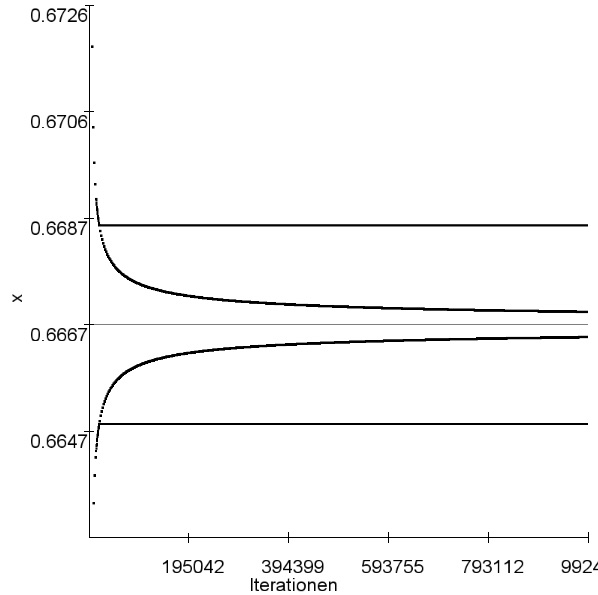
\includegraphics[scale=0.3]{log-konv-r3}
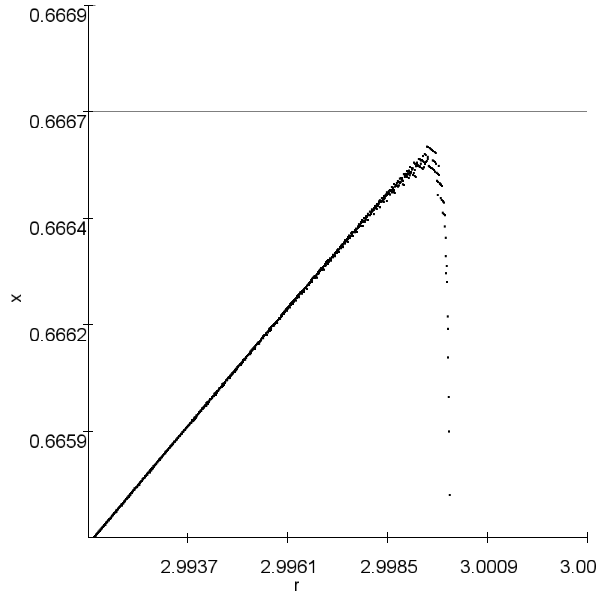
\includegraphics[scale=0.3]{log-bifurc-umr3}
\caption{Links: Konvergenzverhalten der logistischen Abbildung bei $r=3$ untersucht mit zwei Methoden. OpenCL Berechnung: Nach ca. $1.6 \cdot 10^4$ konstant bei $x_n=0.6685$, bzw. $x_{n+1}=6648$. Python Berechnung: $x$ konvergiert kontinuierlich gegen $x=\frac{2}{3}$. Rechts: Vergrößerung des Bifurkationsdiagrammes bei $r\approx3$. $x$ nach $10^5$ Iterationen aufgetragen.}. 
\label{fig:log-konv1}
\end{figure}[!htbp]
Der Bereich um den Bifurkationspunkt ist in Abbildung \ref{fig:log-konv1} (rechts) dargestellt. Dabei wurde zunächst OpenCL für die Berechnung verwendet, was zu einem ungenauem Ergebnis führt. Es lässt sich nur Grob ablesen, dass bei ca. $r=3$ der Fixpunkt $x_1$ instabil ist.
\subsection{Betrachtung von Extremwerten}
Das Bifurkationsdiagramm scheint ab $r>4$ zu divergieren. Im folgenden haben wir diesen Bereich näher analysiert. 
Wegen  $x^2 < x \forall x \in (0,1)$ ist schnell klar, dass sobald $f(I) = [0,1)$ auch $f^n(I) = [0, 1)$. 
Falls aber gilt $x-x^2 < 0$ dann stellt man fest:
\begin{equation}
f^n(x) < ... < f^{2}(x) < f(x) < 0 \forall n \in \mathbb{N} \Rightarrow \lim_{n \rightarrow \infty} f^n(x) = -\infty
\end{equation}
Damit dieses Verhalten irgendwann einsetzt muss gelten: $\exists m: f^m(x) > 1$ denn dann ist $f^{m+1}(x) < 0.$ (wegen $x^2 > x \forall x > 1$). 

\begin{equation}
f(x_0) > 1 \iff x_0-x_0^2 > \frac{1}{r} \iff x_0 = \pm \sqrt{\frac{1}{4}-\frac{1}{r}} + \frac{1}{2}
\end{equation}
Also $\exists x_0 \in \mathbb{R} \forall r > 4: f(x_0) > 1 \Rightarrow f^2(x_0) < 0$ ist. Es ist also zu erwarten, dass 

\begin{equation}
\exists m : f^m(x_0) > 1 \Rightarrow
\lim_{n \rightarrow \infty} f^n(x_0) = -\infty \forall x_0 \forall r > 4
\label{eq:extreme-bifurc-final}
\end{equation}
In prak.iteration-log-extreme.py haben wir nun zu den Anfangsbedingungen $x_0=0.4$, $r \in [3.99999, 4.999989]$, $\Delta r = 0.000001$ überprüft wie viele Punkte r nach n Iterationen gegen $-\infty$ divergieren. Dabei haben $n=1, n=10, n=100, n=1000, n=10000$ Iterationen durchgeführt mit folgendem Ergebniss.

\begin{lstlisting}
python -m prak.iteration-log-extreme
nothing at N_ITER=1
nothing at N_ITER=10
N_ITER=100 found 680 intervals. Last interval [4.072665,4.999989]
N_ITER=1000 found 17 intervals. Last interval [4.000251,4.999989]
N_ITER=10000 found 1 intervals. Last interval [4.000001,4.999989]
\end{lstlisting}

Je mehr Iterationen durchgeführt werden, desto mehr Punkte divergieren ab $r \geq 4.000001$ gegen $-\infty$. Dieses Verhalten war nach Gleichung (\ref{eq:extreme-bifurc-final}) zu erwarten. 

\subsection{Lyapunov Exponent}
Der Lyapunov Exponent beschreibt mit welcher Geschwindigkeit sich zwei naheliegende Punkte voneinander entfernen. 
Es gibt drei Wege den Lyapunov Exponenten zu implementieren:
\begin{equation}
Definition: \lambda(x_0) = \lim_{N \rightarrow \infty}\lim_{\epsilon \rightarrow 0} \frac{1}{N}\log{\mid \frac{f^N(x_0+\epsilon)- f^N(x_0)}{\epsilon} \mid} 
\label{eq:lyapunov-def}
\end{equation}
\begin{equation}
Analytisch: \lambda(x_0) = \lim_{N \rightarrow \infty} \frac{1}{N} \sum_{i=0}^{N-1}  \log{f'(x)} 
\label{eq:lyapunov-analytisch}
\end{equation}
\begin{equation}
Renormiert
\label{eq:lyapunov-renormiert}
\end{equation}
In Abbildung \ref{fix:log-detail} ist der Lyapunov Exponent der analytischen Implementation gezeigt.
Es zeigte sich, dass die Gleichung (\ref{eq:lyapunov-def}) sehr schlechte Ergebnisse im Vergleich zu den beiden letzten Methoden (\ref{eq:lyapunov-analytisch}), (\ref{eq:lyapunov-renormiert}) ergibt.
Dies liegt daran, dass schon bei kleinen $\epsilon$ die Funktionswerte sehr schnell divergieren und somit die Definition des Differenzenquotienten in (\ref{eq:lyapunov-def}) keinen Sinn ergibt.
In Abbildung \ref{fig:lyapunov} (links) haben wir für $r=0.5$ das Konvergenzverhalten von (\ref{eq:lyapunov-def}) mit dem Konvergenzverhalten von (\ref{eq:lyapunov-analytisch}) verglichen. Es ist zu sehen, dass an $N=60$ der Differentialquotient beginnt von der analytischen Version abzuweichen und schließlich bei $N=125$ divergiert.
Die Renomierung (\ref{eq:lyapunov-renormiert}) hält diesen Abstand in jedem Iterationsschritt klein, weshalb sich der Lyapunov Exponent trotzdem ausrechnen lässt.
Der Lyapunov Exponent hat $\lambda(x_0)$ seine Nullstellen dort wo die Abbildung ihre periodenverdoppelnden Stellen hat. Umgekehrt divergiert $\lambda(x_0)$ an den superattraktiven Stellen gegen $-\infty$.
Man erhält also Information über das Verhalten der Abbildung für bestimmte $x_0$.
Tatsächlich kann man den Lyapunov-Exponenten über den mittleren Informationsverlust ausdrücken $\lambda(x_0)=-log(2)*\delta I$ (QUELLE skript todo).
Im folgenden ist der OpenGL Quellcode der renomierten Formel des Lyapunov Exponenten gezeigt:
\begin{lstlisting}
float g(float r, float x) {
    return r * x * (1-x);
}
vec4 f(vec4 x) {
    float x0 = 0.4;
    float eps = 0.0001;
    float n = 10000;
    float summe = x0;
    for (int i=1; i < n; i++) {
        x0 = g(x.x, x0);
        summe += log(abs(g(x.x, x0+eps)-g(x.x, x0))/eps);
    }
    return vec4(x.x, summe/n, 0, 0.5);
}
\end{lstlisting}
\subsubsection{Konvergenzverhalten}
Es kann passieren, dass man einen Anfangswert wählt, für welchen der Lyapunov-Exponent kein sinnvolles Ergebniss liefert. Setzt man $x_0=0.5$ so divergiert die analytische Formel, denn $log(f'(x_0))=-\infty$.
Für die renormierte und analytische Implementation haben wir untersucht wie schnell bestimmte Anfangswerte $x_0$ gegen den Grenzwert $\lambda(x_0)$ streben. Dafür wurde untersucht wie nah $\lambda_{N=5}(r, x_0)$ an $\lambda_{N=1000}(r, x_0)$ ist:
\begin{equation}
    \gamma = exp^{-500 * (\lambda_{N=5}(r,x_0)
    - \lambda_{N=10000}(r,x_0))^2}
\end{equation}
In Abbildung \ref{fig:lyapunov} ist das Ergebniss zu sehen: Je dunkler ein Punkt (r, $x_0$) ist, desto besser konvergiert $\lambda(r, x_0)$ ($\gamma \approx 1$). 
Es gibt also $x_0$ welche ein sehr schnelles Konvergenzverhalten gegenüber anderen $x_0$ haben. Der oben besprochene Startwert $x_0=0.5$ ist in der rechten Abbildung gut bestätigt, denn hier konvergiert $\lambda(r, x_0)$ nicht. 

\begin{figure}[!htbp]
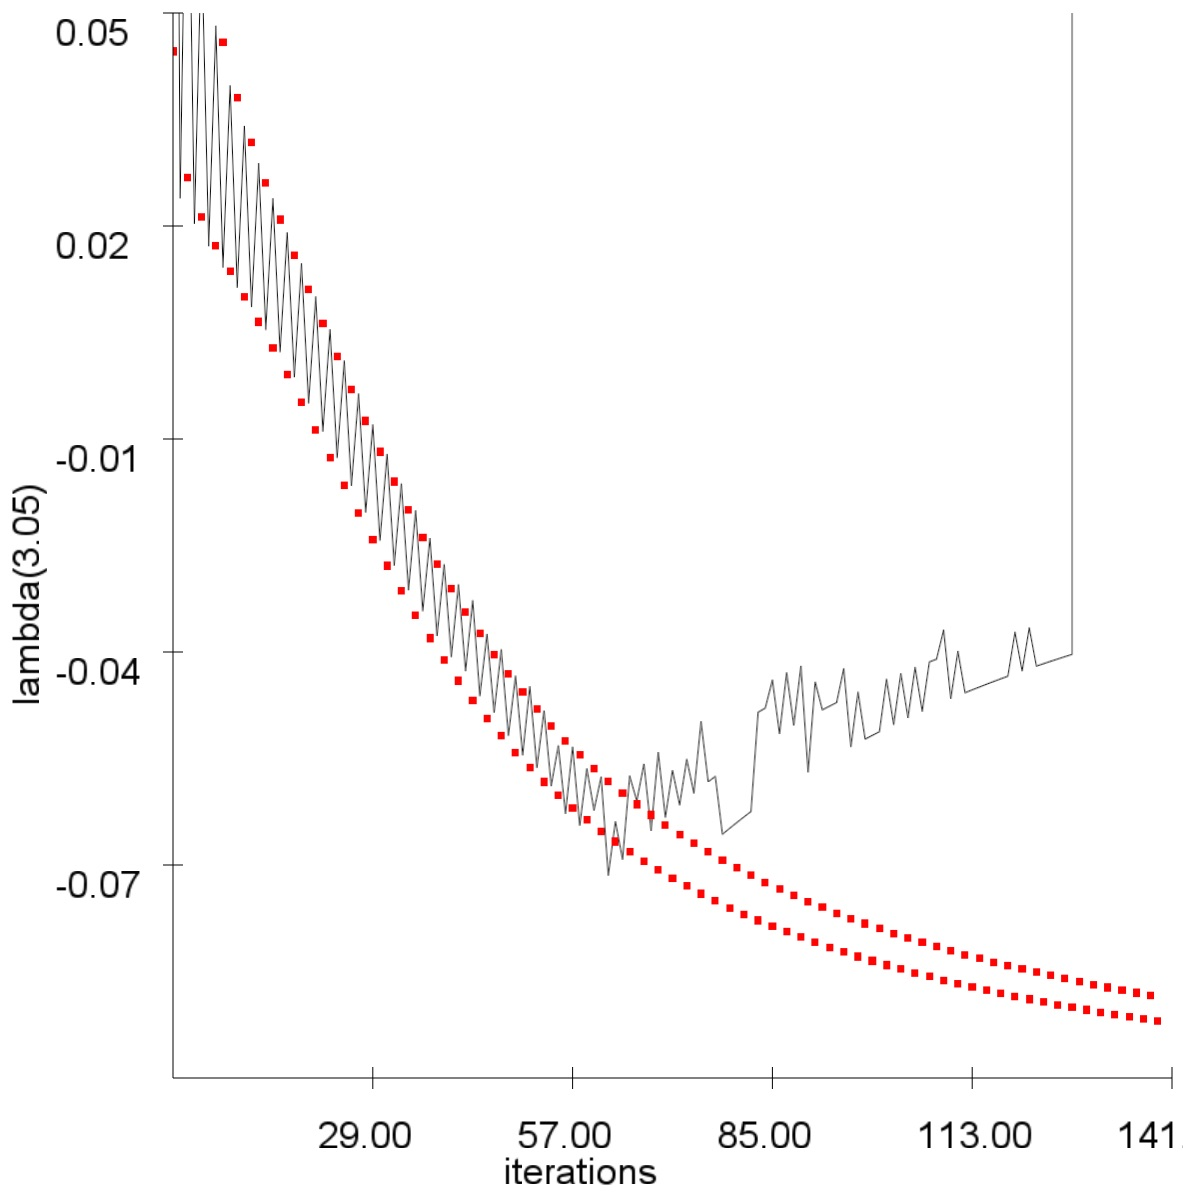
\includegraphics[height=160px]{lyapunov-definition-convergence}
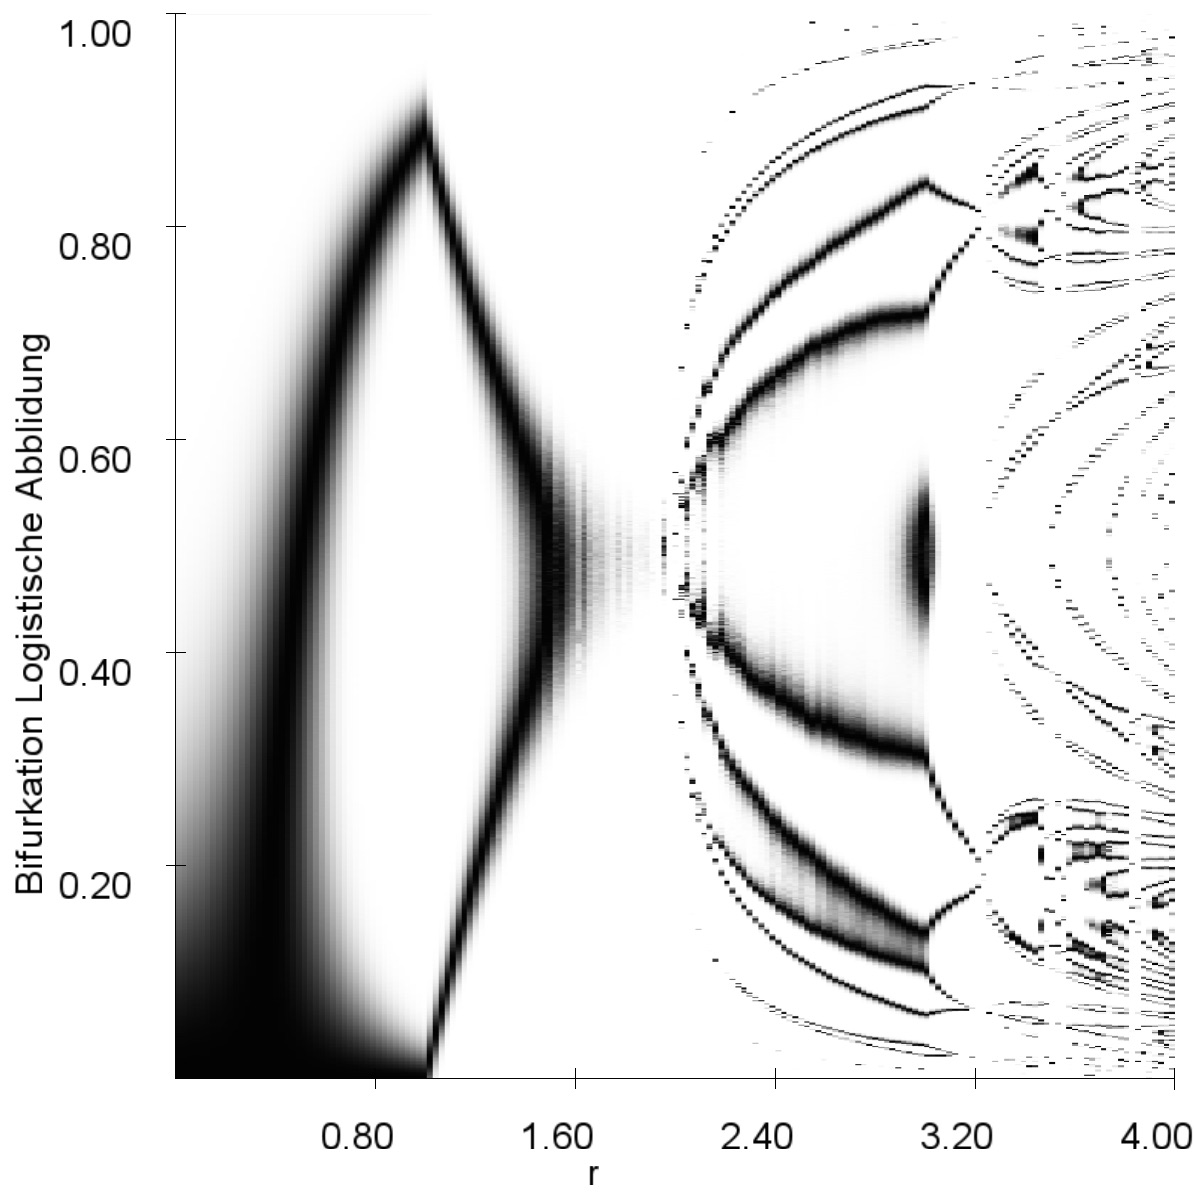
\includegraphics[height=160px]{lyapunov-normiert-xr}
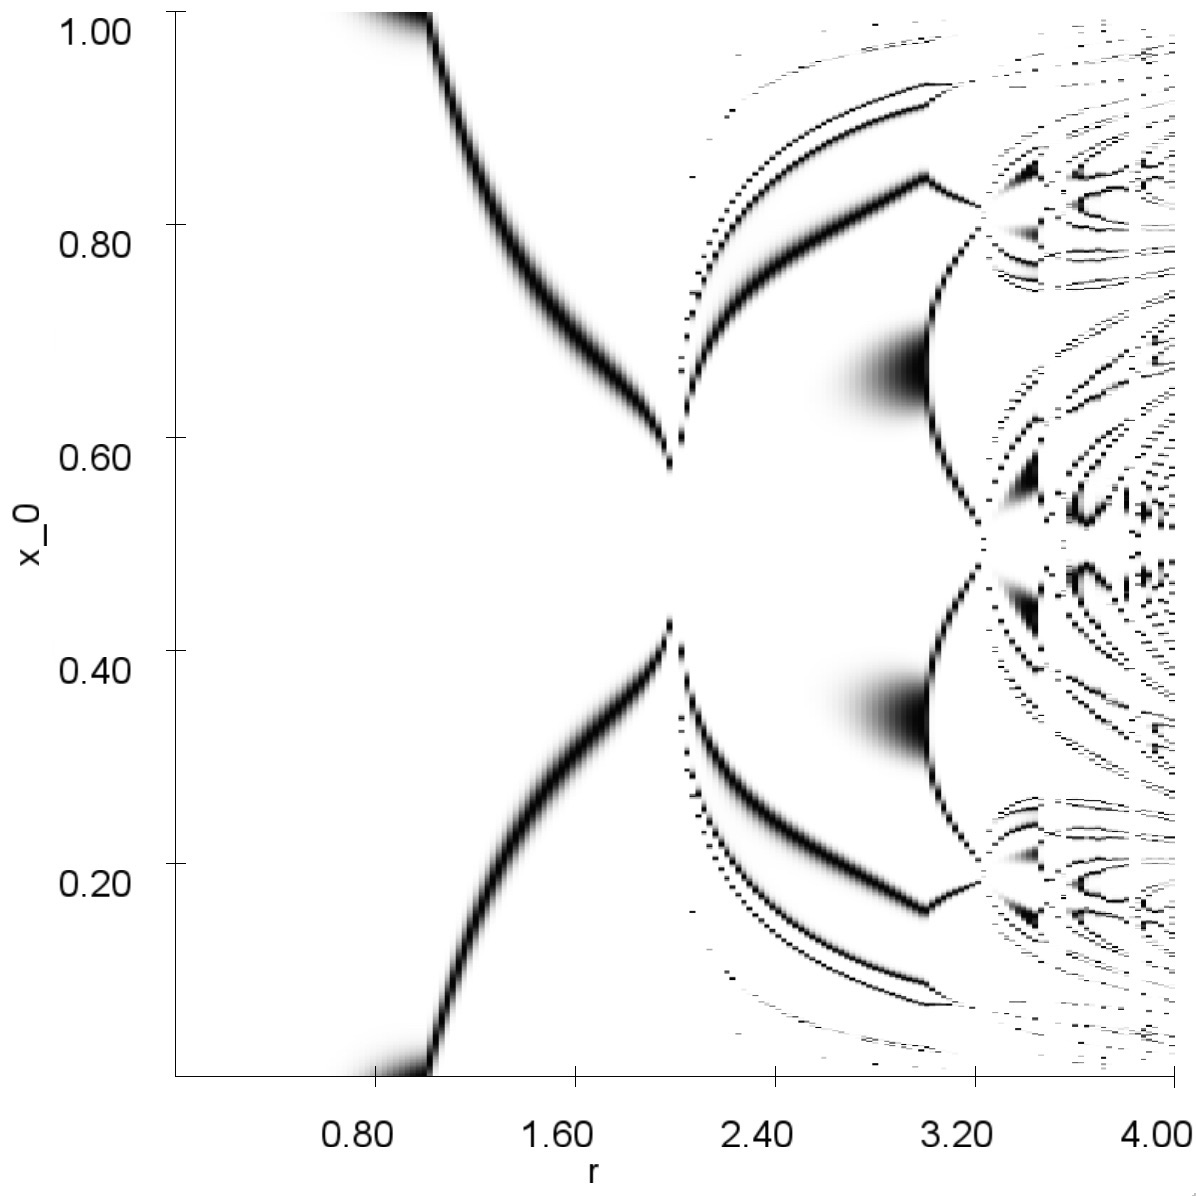
\includegraphics[height=160px]{lyapunov-analytisch-xr}
\caption{Analyse des Lyapunov Exponenten. Links: Konvergenz der analytischen Implementation (Punkte) gegen Konvergenz der Definition (Linie, zu besseren Visuellen Unterscheidung wurden die diskreten Abbildungspunkte Verbunden). Mitte: Kontrollparameter r aufgetragen gegen Definitionsbereich $x_0$. Je dunkler ein Punkt (r, $x_0$) desto besser konvergiert $\lambda(r,x_0)$. Rechts: Analog zur Mittleren Abbildung für die analytische Implementation (sourcecode: prak/lyapunov-defintion-convergence.py, prak/lyapunov-rx-convergence.py)} 
\label{fig:lyapunov}
\end{figure}
 
\subsubsection{Betrachtung im chaotischen Bereich.}
In Abbildung \ref{fig:lyapunov} ist zu sehen wie der Lyapunov Exponent ab $r=3.56$ nicht mehr stetig konvergiert. 
Der Verdacht liegt nahe, dass nicht genügend Iterationsschritte zur Berechnung ausgeführt wurden also erhöhten wir die Anzahl an Iterationsschritten für die Berechung von $\lambda(x)$. Es zeigte sich allerdings kaum eine Veränderung. Die Frage nach der Konvergenz von $\lambda(x)$ im chaotischen Bereich galt es zu untersuchen: Abbildung \ref{fig:lyapunov-chaos} zeigt das Langzeitverhalten von $\lambda(x)$ über $19*10^6$ Iterationen. $\lambda(x)$ erinnert die ersten $10^7$ Iterationen eher an einen Börsenkurs als ein Objekt welches gegen einen Grenzwert konvergiert. Erst nach ca. $10^7$ Iterationen deutet sich Konvergenzverhalten an. Dieses ist aber nicht präzise: Falls 
\begin{equation}
\lim_{N \rightarrow \infty} \lambda_N(x) = L
\end{equation}
so kann man nach $2*10^7$ Iterationen höchstens feststellen, dass der Graph in einen Epsilon Schlauch von $\epsilon=0.002$ passt. Dies ist nicht sehr befriedigend angesichts der massiven Iterationslänge.  
 
\begin{figure}[!htbp]
\centering
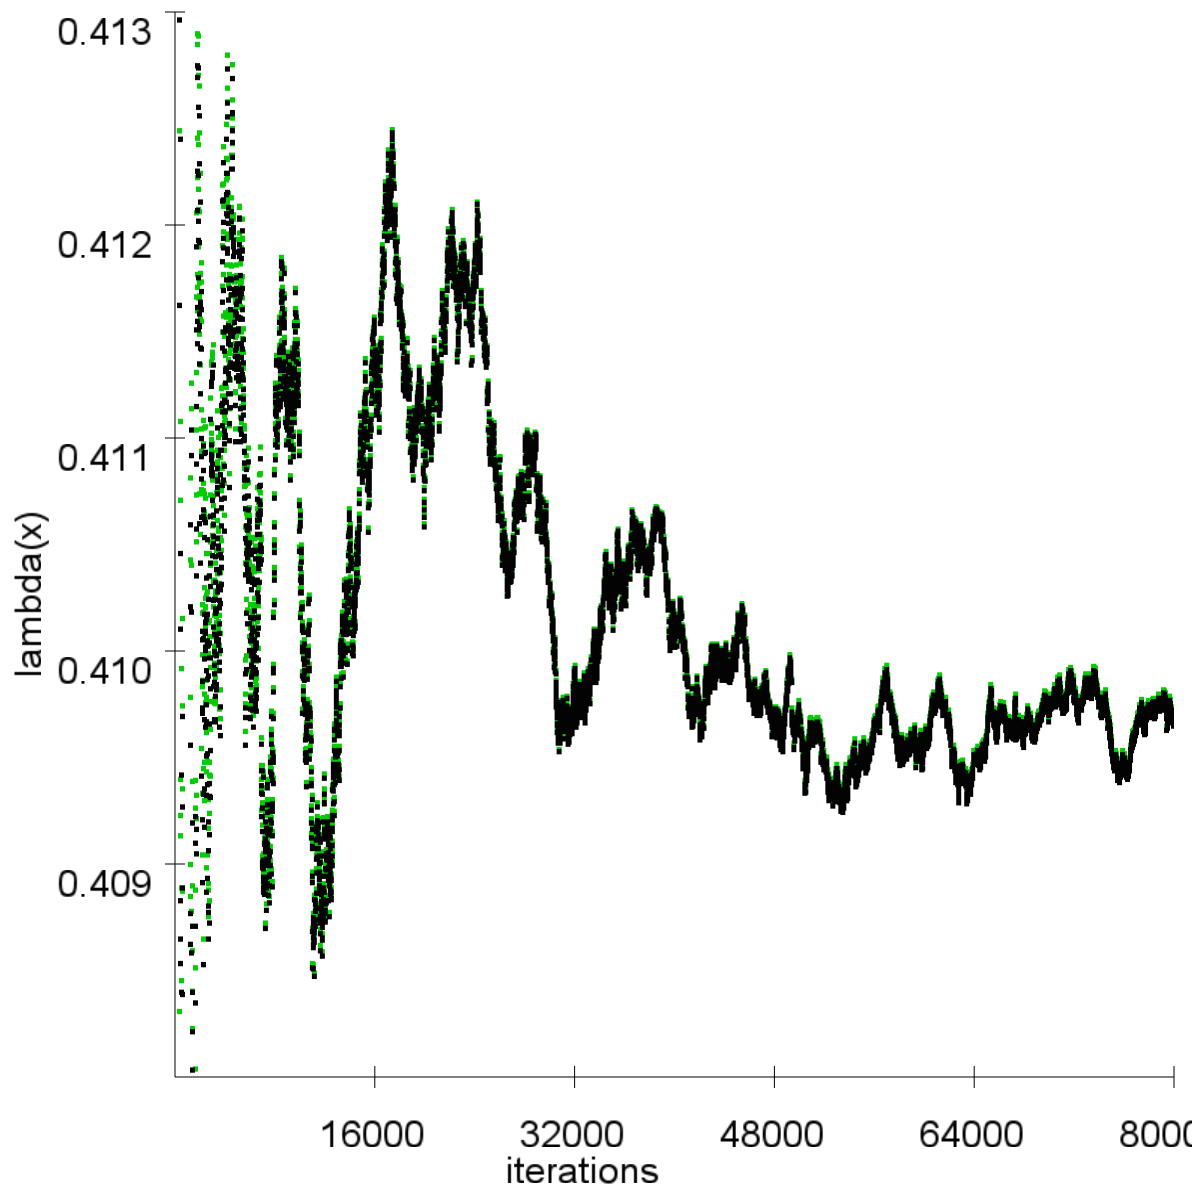
\includegraphics[height=150px]{lya378-zoom}
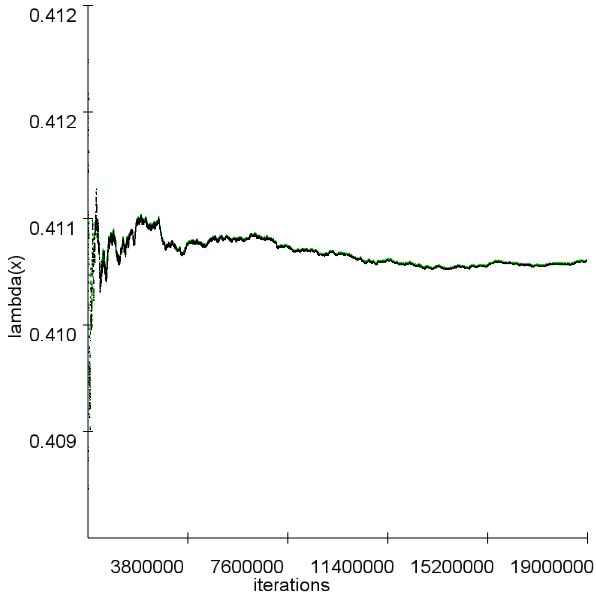
\includegraphics[height=150px]{lya378}
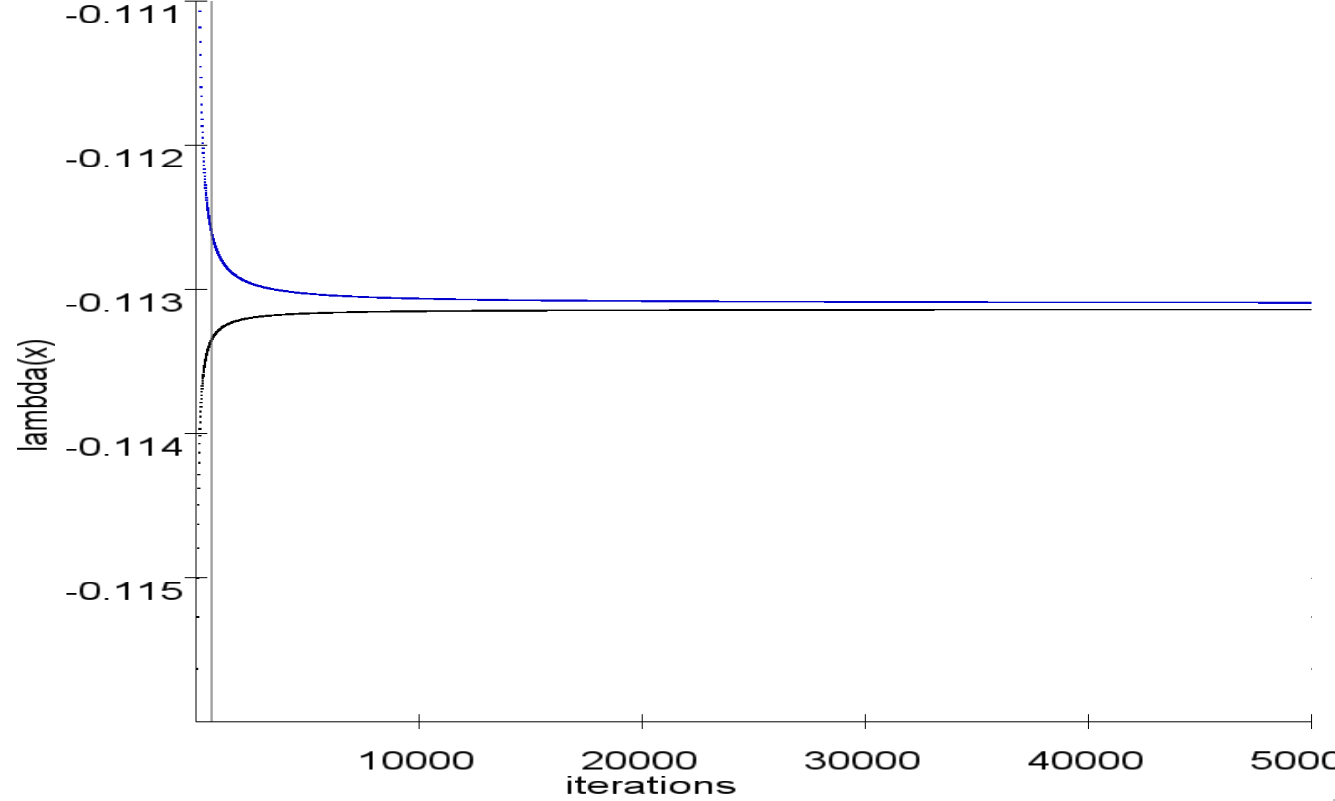
\includegraphics[height=150px, width=150px]{lyapunov-analysis-305}
\caption{Analytischer(schwarz) und renormierter(grün) Lyapunov Exponent im chaotischen Bereich bei $r=3.78$. Mitte: Zoom im Bereich 0 bis $80*10^3$ Iterationen. Rechts:  0 bis $19*10^6$ Iterationen.
Rechts: Vergleich des analytischen(Schwarz) und renormierten(Blau) Iterationsverhalten des Lyapunov Exponenten bei $r=3.05$. Vertikale Linie bei N=700. }
\label{fig:lyapunov-chaos}
\end{figure}


\subsubsection{Vergleich der analytischen und renomierten Implementation}
Wir haben nun die analytische und die renormierte Implementation des Lyaponovexponenten weiter untersucht. Dabei stellten wir fest, dass bei Stellen mit Periodenverdoppelung die renormierte Formel etwas schneller gegen 0 konvergiert als die analytische Formel. An einer weiteren Stelle ($r=3.05$) ist zu erkennen wie beide Implementationen jeweils von oben (renormiert) und von unten (analytisch) gegen einen gemeinsamen Wert streben (Abbildung \ref{fig:lyapunov-chaos}). 
Die Vermutung liegt nahe, dass man mit dem Mittelwert aus beiden Implementationen an solchen stellen wesentlich schneller den Grenzwert bestimmen kann. Es zeigt sich aber, dass dieses Verhalten nicht regelmäßig auftritt weshalb wir es nicht weiter untersucht haben. Nach weiteren Stichproben scheint die analytische Implementation bis zum 500ten Iterationsschritt etwas schneller als die renormierte Implementation zu konvergieren. Beide Versionen zeigten in allen Stichproben $r<3$, dass sie stets gegen den gleichen Grenzwert strebten.


\subsection{Feigenbaumkonstante}
Die Feigenbaumkonstante ist eine universelle Größe. Sie tritt in chaotischen nicht linearen System auf und ist definiert:
\begin{equation}\delta_i = \frac{b_i-b_{i+1}}{b_{i+1}-b_{i+2}}=\frac{s_i-s_{i+1}}{s_{i+1}-s_{i+2}}\end{equation}
\begin{equation}\delta = \lim\limits_{i \rightarrow \infty}{\delta_i} = 4.669201609102991\end{equation} 
(TODO QUELLE https://oeis.org/A006890)
wobei $s_i, b_i$ die Folgen der superattraktiven und periodenverdoppelden Stellen sind.
Also lässt sich die Feigenbaumkonstante mit dem Lyapunov Exponenten bestimmen. 
Als erstes haben wir versucht die Nullstellen des Lyapunov Exponenten zu bestimmen. Wir wendeten dabei das folgende Kriterium für Nullstellen an:
\begin{equation}
\lambda(x-\epsilon) < \lambda(x) \wedge \lambda(x+\epsilon) < \lambda(x) \wedge |\lambda(x)|<\epsilon
\end{equation}
Bei genauer Betrachtung des numerisch bestimmten Lyapunov Exponenten zeigten sich große Schwankungen, weshalb dieses Kriterium nicht mit unseren Verfügbaren Rechenleistungen praktikabel war (Abbildung \ref{fig:lya-rauschen}).
Aufgrund dieser Probleme
haben wir uns dazu entschieden die superattraktiven Stellen anstelle der Bifurkationspunkte numerisch zu bestimmen. Unser Algorithmus startet im Suchmodus bei gegeben Startwert $x_{start}$ und geht in kleinen Schritten $\Delta x$ die x-Achse ab. In jedem Schritt wird $l_1=\lambda(x_0)$ $l_2=\lambda(x_0 + \Delta x)$ berechnet. 
Ist
\begin{equation}
l_2-l_1 \leq 0 
\label{eq:bedinung-1}
\end{equation}
wandert der Iterationsschritt zum superattraktiven Fall. 
Dies wird so lange fortgesetzt bis die Bedingung (\ref{eq:bedinung-1}) nicht mehr hält. 
Es wird nun um $\Delta x$ zurückgegangen und anschließend die Schrittweite $\Delta x \mapsto \frac{\Delta x}{10} $ verkleinert. Nun wird erneut so lange iteriert, bis (\ref{eq:bedinung-1}) nicht mehr hält. 
Der Vorgang wiederholt sich 8 mal. Anschließend wird $(2*x_0 + \Delta x )/2$ als Ergebniss gespeichert. 
Als nächstes befindet sich der Algorithmus im Anfangspunkt-Modus. Es wird so lange die x-Achse abgetestet bis die Bedingung 
\begin{equation}
\lambda(x_0) < \lambda(x_0 + \Delta x) < \lambda(x_0 + 2*\Delta x)
\end{equation}
nicht mehr erfüllt ist und somit ein neues $x_{start}$ gefunden wurde. Der Suchmodus wird aktiviert  (Quellcode: prak/feigenbaum.py).
Im folgenden ist die Terminal Ausgabe des Algorithmusses beigelegt:
\begin{lstlisting}
searching from 1.9
looking for next start_r from 2.00000000002
searching from 2.99950000003
looking for next start_r from 3.23606797751
searching from 3.44927797752
looking for next start_r from 3.49856169934
searching from 3.54400769935
looking for next start_r from 3.55464086278
searching from 3.56439786279
looking for next start_r from 3.56666737986
found values [2.0000000000249916, 3.236067977509959, 3.498561699344952, 3.554640862779951, 3.5666673798649517]
delta_0=4.70894301336
delta_1=4.68077099865
delta_2=4.66295961155
\end{lstlisting}
Somit konnten wir numerisch für $i=2$ eine Feigenbaumkonstante von $\delta_2=4.66295961155$ berechnen. Dieser Wert weicht um 0.12\% vom tatsächlichen Wert ab. Die Grenzen des Algorithmus sind bereits nach 5 gefunden superattraktiven Stellen erreicht. Ab $r>3.57$ fängt die numerische Implementation des Lyapunov Expontenten an zu "rauschen" (Abbildung \ref{fix:log-detail}). Der Algorithmus kann daher nicht mehr präzise seinen Suchmodus ausführen. Ebenfalls liegen die nächsten superattraktiven Punkte noch dichter zusammen als es für $s_4$, $s_5$ der Fall war, was ebenfalls vom Algorithmus nicht mehr detektiert wird. 
\begin{SCfigure}
\centering
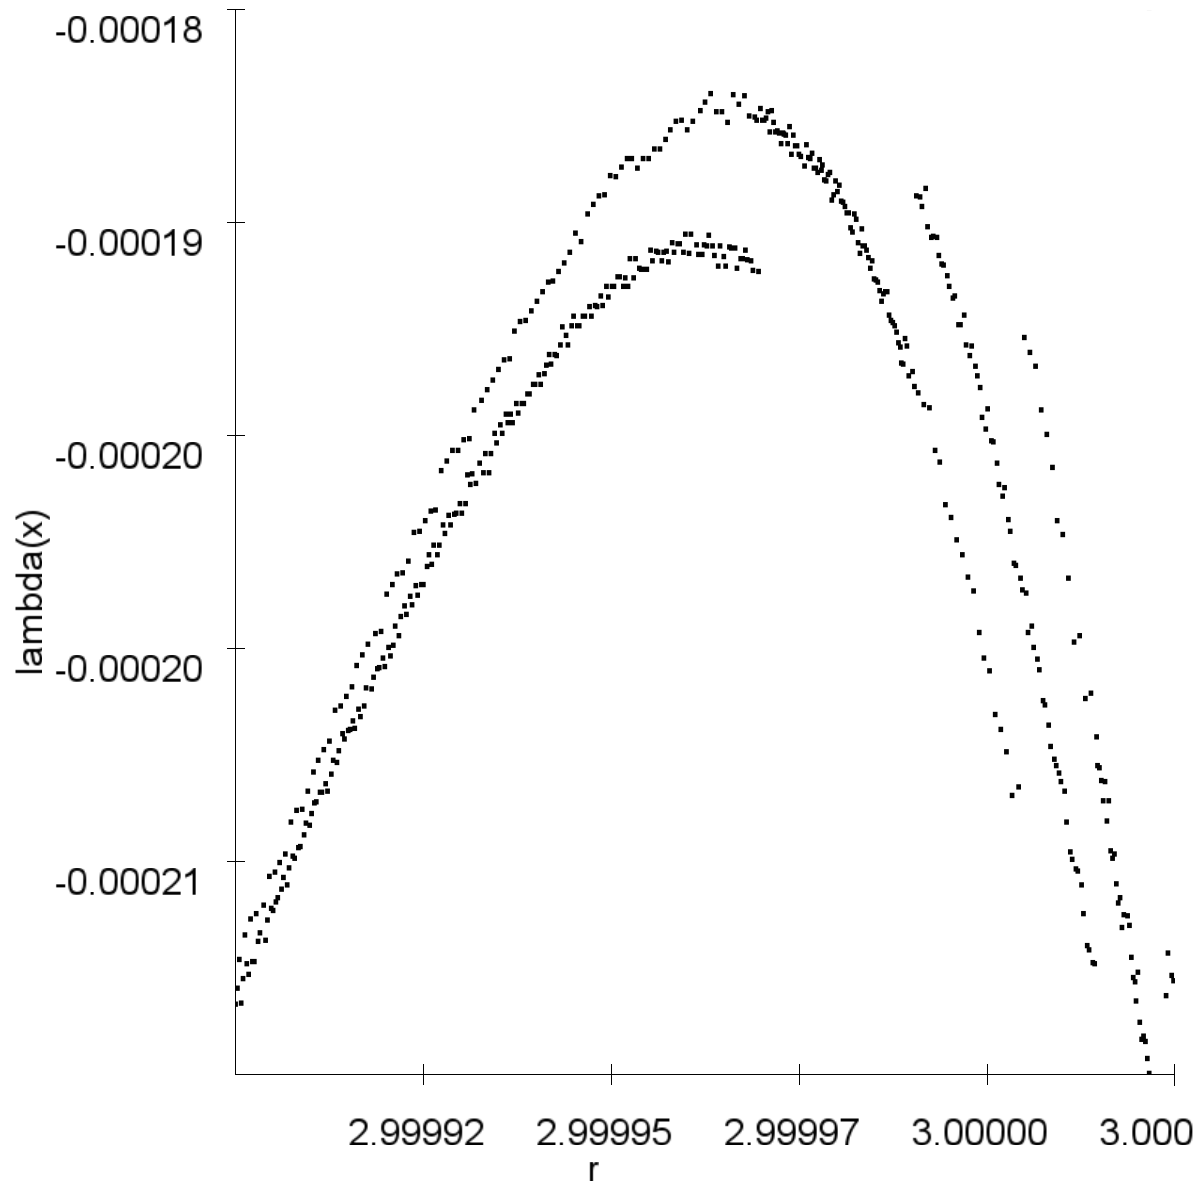
\includegraphics[scale=0.20]{lya-rauschen}
\caption{Zoom in den Lyapunovexponenten der logistischen Abbildung bei $r=3$ mit 80000 Iterationen. 
Eine präzise Konvergenz ist nicht zu erkennen wodurch die numerische Bestimmung der Spitzen an den Bifurkationspunkten erschwert wird. Sourcecode: prak/lyapunov-superattraktiv.py}. 
\label{fig:lya-rauschen}
\end{SCfigure}



\begin{figure}[!htbp]
\centering
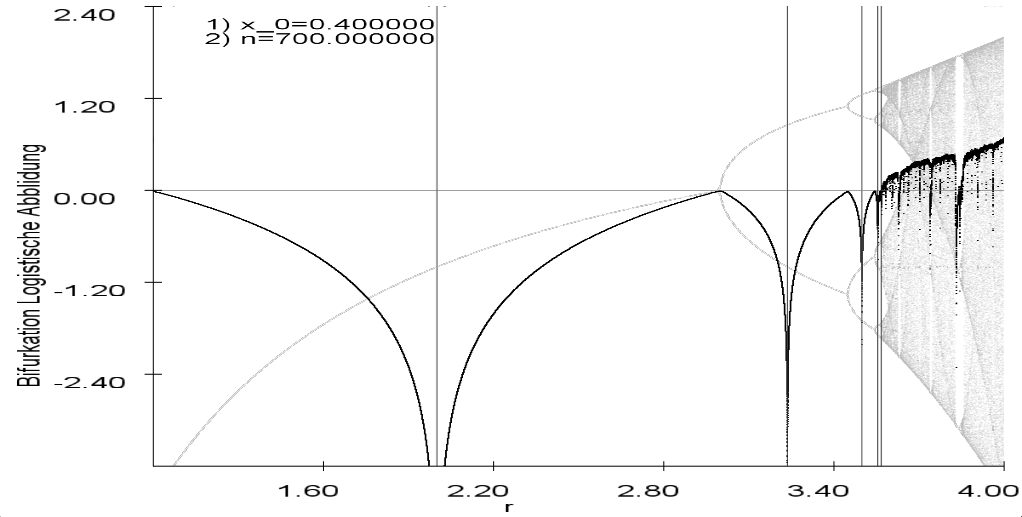
\includegraphics[scale=0.45]{iteration/bifurk-log-lyapunov-periode}
\caption{Analyse des Bifurkationsdiagrammes der logistischen Abbildung. Eingezeichnet sind die y=0 Achse, sowie die ersten 5 Superattraktiven Stellen. Das Bifurkationsdiagramm wurde so translatiert und skaliert, so dass es hinter dem Lyapunov Exponenten erscheint.}.
\label{fix:log-detail} 
\end{figure}







\section{Sinus Abbildung}
Die Sinusabbildung ist gegeben durch 
$$f(x_n)=x_{n+1}=r*sin(x)$$
Wir haben die bereits implementierten Programme nun auf die Sinus Funktion angewendet. Abbildung \ref{fig:bifurc-sin} zeigt das Bifurkationsdiagramm der Sinusabbildung. Es fällt sofort auf, dass sich die Bildpunkte innerhalb einer Einhüllenden befinden. Betrachtet man die Funktion wird wegen des Bildbereiches des Sinus ($[-1,1]$) sofort klar, dass $\sup_{n \in \mathbb{N}} |f^n(r)| \leq r $ gilt. Bei den Bifurkationsdiagrammen der logistischen Abbildung hatten wir ein festen Startwert $x_0$ gewählt. Für die Sinusabbildung wählten wir als Startwerte die Folge $x_{0,n} = (-1)^n * x_0$ da sonst im Bereich $r \in [0,\pi]$ das Bild des Graphen stets positiv wäre. Auch dieses Phänomen lässt sich mit einfachen Überlegungen erklären: 
$$sin([0,\pi]) = [0,1] \Rightarrow f([0,\pi]) = [0,\pi] \Rightarrow f^2([0,\pi]) = [0,\pi] \forall r \in [0,\pi]$$
 
Das Anwenden unseres Algorithmus zur bestimmung der Feigenbaumkonstante lieferte im Vergleich zur logistischen Abbildung keine guten Ergebnisse. Die ersten superattraktiven Stellen $s_i$ ließen sich ohne weiteres bestimmen. Die Abstände $\Delta s$ werden schon nach den ersten 4 Folgegliedern sehr klein und der Lyapunov Exponent beginnt zu "rauschen". 
Wir entwickelten einen weiteren Algorithmus, welcher nur marginal bessere Ergebnisse nach $s_4$ lieferte. Die Idee des Algorithmusses war es, zunächst den Lyapunov Exponenten Grob für $r\in [0,3.2]$ zu berechnen. 
Die so entstandene Folge $l_i=(x_i, l(x_i))$ wird nun iteriert. Sobald $l_{i,1} < M < 0$ gilt wird $A=l_{i,0}$ gesetzt. Es wird weiter iteriert bis $l_{i,1} > 0$ und schließlich wird das Intervall $[A, l_{i,1}]$ gespeichert. Dies wird bis zum Ende der Folge $l_i$ ausgeführt. 
Nun wird der Algorithmus für eine tiefere Schranke auf alle ermittelten Intervalle erneut angewendet. 
Wir fanden so mehrere Hinweise für die nächsten superattraktiven Stellen. 
Schließlich wurde $M \leq 4.0$ und plötzlich fielen keine Punkte außer $s_1, s_2, s_3, s_4$ in das Raster. Beim betrachten des Lyapunovexponenten fiel auf, dass trotz einer Iterationstiefe von 10000 Iterationen stets galt $\lambda(x)>-4.0$. 
Wir haben dafür nur zwei plausible Erklärungen: 
(1.) $s_5-s_4$ ist sehr klein und wir erwarten, dass $s_6-s_5$ noch kleiner ist (untere Abbildung \ref{fig:bifurc-sin}): Eventuell reicht unsere numerische Genauigkeit nicht aus. 
(2.) Der Sinus ist ungenau implementiert und verschmiert so den Grenzwert. 
Die folgenden superattraktiven Stellen haben wir ermittelt: $s_1=0.0$, $s_2=1.570728749999546$ $s_3=2.4432446071429674$, $s_4=2.6580499999998904$, $s_5=2.70599999999986$, $s_6=2.71600010303040$ und daraus die ersten 4 Glieder in der Feigenbaum Folge bestimmen:
$$\delta_1=1.8002294596$$
$$\delta_2=4.06188990667$$
$$\delta_3=4.47977878743$$
$$\delta_4=4.79495059736$$

Anders als die logistische Abbildung bricht das Bifurkationsdiagramm der Sinusfunktion nicht ab. Auch dies lässt sich auf den Kompakten Bildbereich des Sinus zurückführen. Der Lyapunov Exponent weist ab $r>8$ eine Perdiodizität von $\pi$ auf weshalb weitere Betrachtungen für $r>8$ nicht zielführend erscheinen.

\begin{figure}[!htbp]
\centering
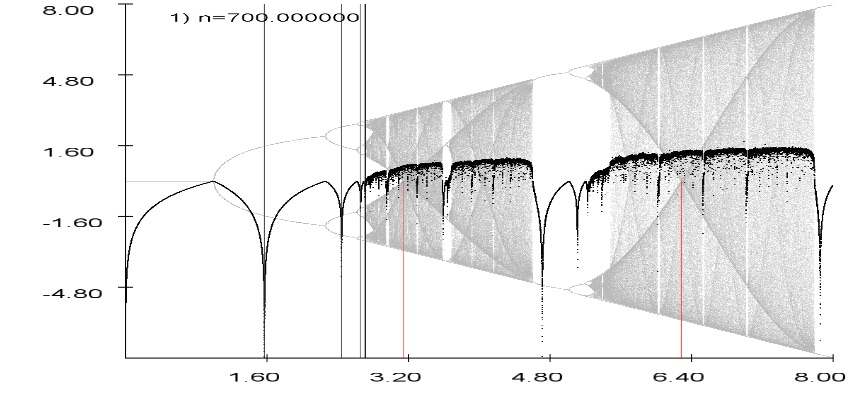
\includegraphics[height=220px, width= 220px]{bifurkation-sin}
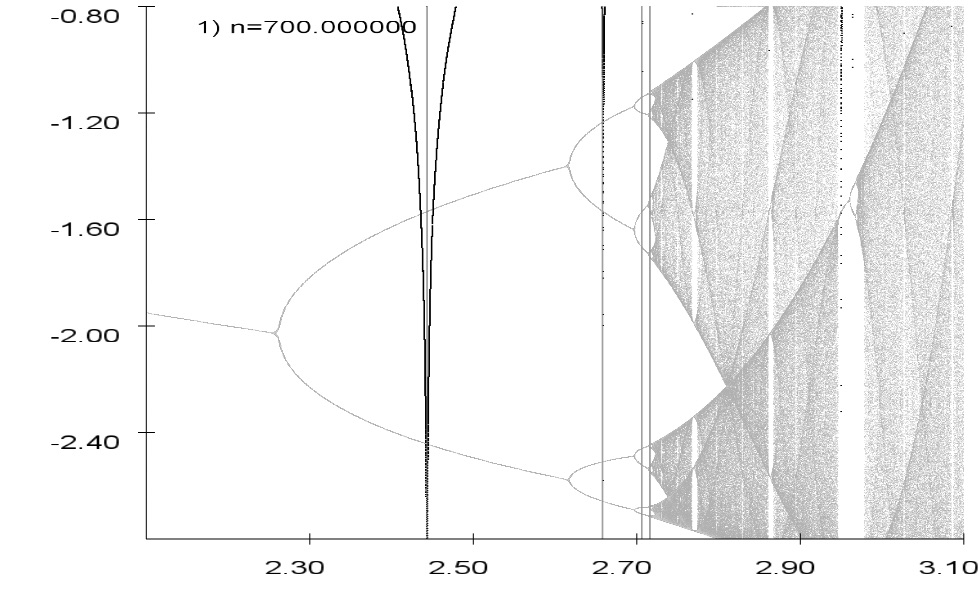
\includegraphics[height= 220px, width= 220px]{bifurkation-sin-zoom}
\caption{Links: Analyse des Bifurkationsdiagrammes der sinus Abbildung. Eingezeichnet sind die ersten 6 Superattraktiven Stellen (Erste Superattraktive Stelle bei $r=0$. Ebenfalls wurden $\pi$ und $2\pi$ eingezeichnet. Rechts: Vergrößerung des Ausschnittes $r \in [2.1,3.1], y\in[-2.8,-0.8]$}. 
\label{fig:bifurc-sin}
\end{figure}
\newpage
\section { Duffing-Gleichung}
Wir betrachten nun einen angetrieben und gedämpften Oszillator. Als Unterschied zum gewöhnlichen Harmonischen Oszillator wird der Term mit der Federkonstante kubisch. Dies ist vergleichbar mit der Schwingung eines Metallstabes.
\begin{equation}
\ddot{x}+\lambda\dot{x}+\beta x^3=\epsilon\cos{\Omega t}
\label{eq:duffing}
\end{equation} 
Diese DGL lässt sich nun nicht mehr analytisch berechnen.
Im Folgenden lösen wir die Gleichung mit der Euler-Methode \parencite{wiki:euler} als auch mit dem Runge-Kutta Verfahren \parencite{wiki:runge}. Um dies zu ermöglichen lässt sich \eqref{eq:duffing} als folgendes DGL System umformen.
\begin{equation}\frac{dy}{dt}=\epsilon\cos{\theta}-\lambda y - \beta x^3\end{equation}
\begin{equation}\frac{dx}{dt}=y\end{equation}
\begin{equation}\frac{d\theta}{dt}=\Omega\end{equation}
\newline
\subsection { Phasenraumdiagramm }
Im folgenden verwenden wir als Parameter $\epsilon = 0,2$, $\lambda = 0,08$, $\beta = 1$ und $\Omega = 1$ und untersuchen die Unterschiede der verwendeten numerischen Verfahren bei gleich bleibenden Anfangswerten. Dazu wählen wir $x_0=0.21$ und $y_0=0.02$ und betrachten das Phasenraumdiagramm bei unterschiedlichen Schrittgrößen $h$. Für kleine Parameter $h$ erhalten wir sowohl bei dem Euler-Cauchy, als auch beim Runge-Kutta Verfahren (Runge-Kutta 4ter Ordnung 3-Dimensional, siehe Appendix) Attraktoren wie in Abbildung \ref{fig:duffing-awp1} (mitte) dargestellt. 
\begin{figure}[!htbp]
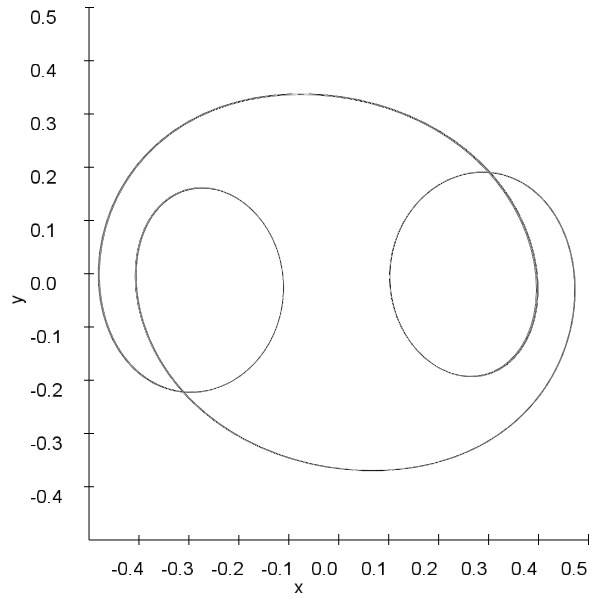
\includegraphics[scale=0.28]{duffing-awp1-500k-nach-500k-h0,1-euler}
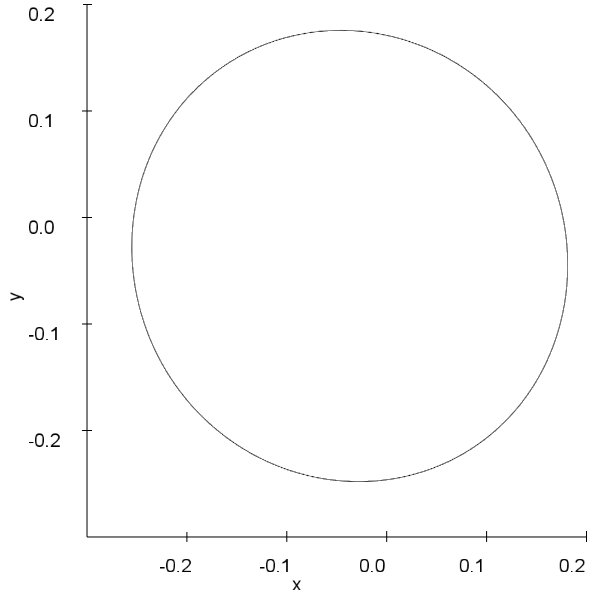
\includegraphics[scale=0.28]{duffing-awp1-500k-nach-500k-h0,08-euler}
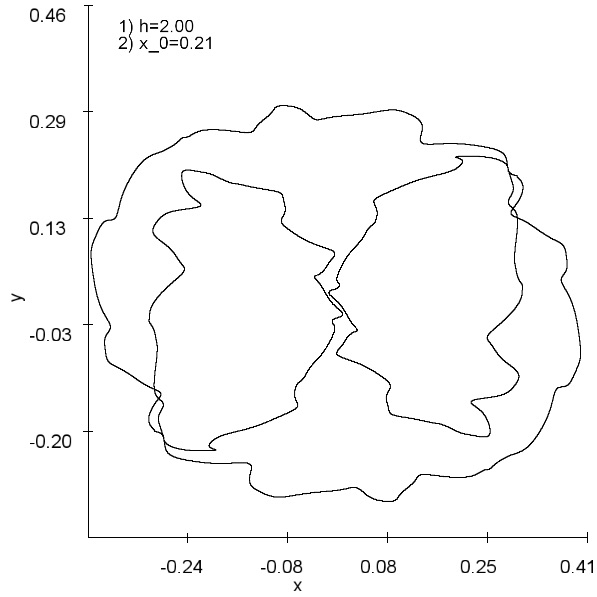
\includegraphics[scale=0.28]{duffing-awp1-h2-runge-kutta}
\caption{Phasenraumdiagramm. Links: Schrittweite $h=0.1$ mit Euler-Cauchy. Mitte: Schrittweite $h=0.08$ mit Euler-Cauchy identisch bei $h=0.1$ mit Runge-Kutta . Rechts: Runge-Kutta bei Schrittweite $h=2$}. 
\label{fig:duffing-awp1}
\end{figure}
Für $0.2<h<0.08$ erhalten wir mit dem Euler-Cauchy Verfahren einen anderen Attraktor (Abbildung \ref{fig:duffing-awp1} links) und für $h>0.2$ divergiert die Trajektorie. Bei dem Runge-Kutta-Verfahren können wir $h>0.2$ wählen und erhalten weiterhin einen Attraktor wie in Abbildung \ref{fig:duffing-awp1} (rechts). Wählen wir noch größere Schrittweiten so beobachten wir plötzlich bei $h=2$ einen Attraktor wie in Abbildung \ref{fig:duffing-awp1} rechts.
\newline
Im weiteren sind alle folgenden Berechnungen in diesem Kapitel mit dem Runge-Kutta-Verfahren 4ter Ordnung gemacht.
\newline
Ganz bedeutend ändert sich der Attraktor, bei Variation der Anfangsbedingungen. Variieren wir $x_0$ so bleibt der Attraktor identisch bei $x_0=0.18$, während wir bei $x_0=0.17$ ein Phasenraumdiagramm ähnlich zu Abbildung \ref{fig:duffing-awp1} (links) erhalten.
\newline
Abbildung \ref{fig:duffing-allawp} zeigt Attraktoren bei unterschiedlichen Anfangsbedingungen.
\begin{figure}[!htbp]
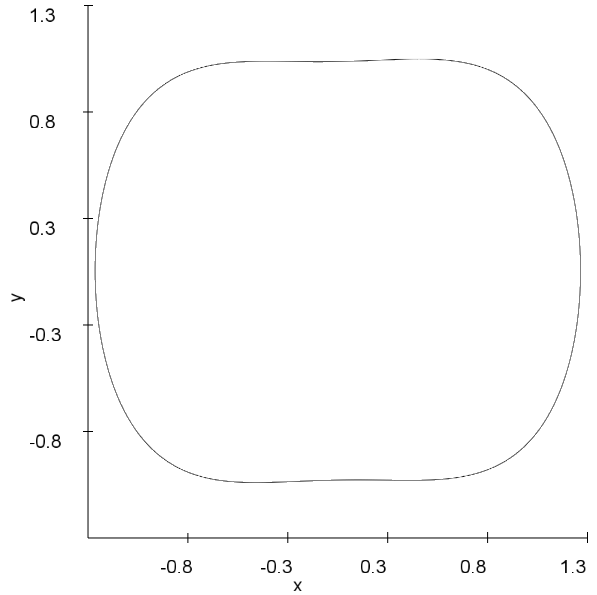
\includegraphics[scale=0.4]{duffing-awp2-500k-nach-500k-h0,01-runge}
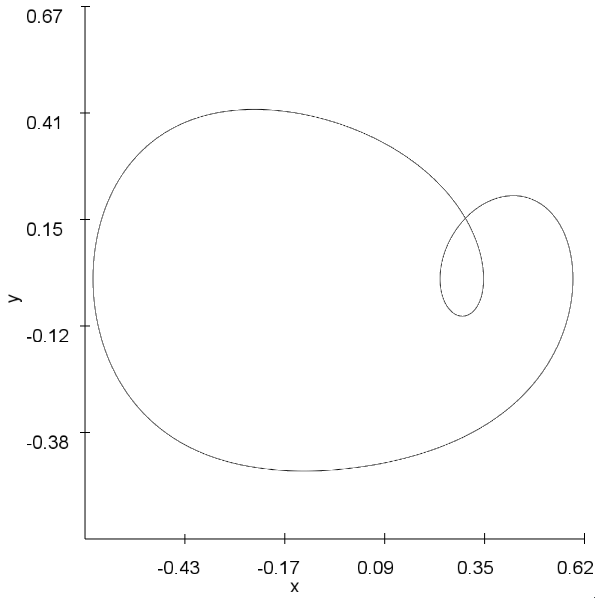
\includegraphics[scale=0.4]{duffing-awp3-500k-nach-500k-h0,01-runge}
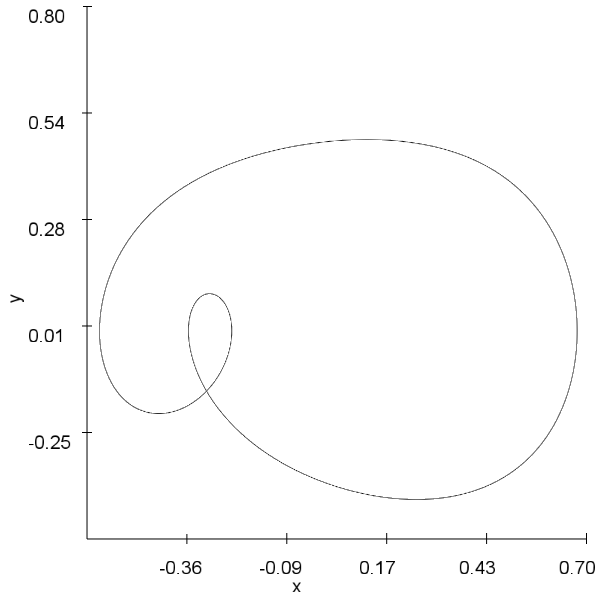
\includegraphics[scale=0.4]{duffing-awp4-500k-nach-500k-h0,01-runge}
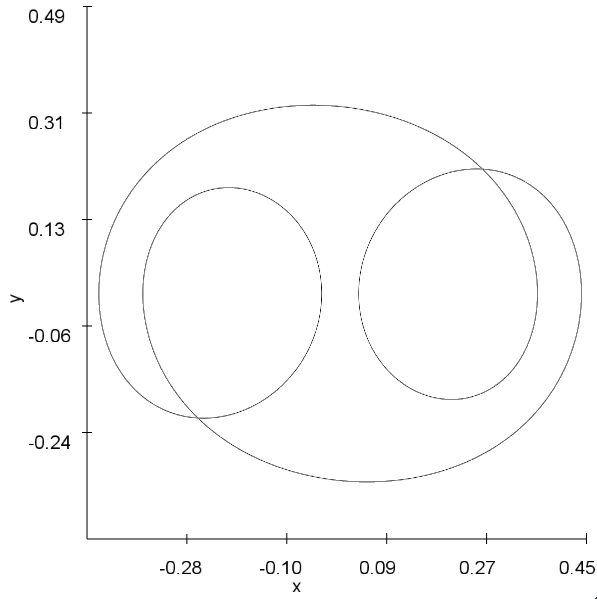
\includegraphics[scale=0.4]{duffing-awp5-500k-nach-500k-h0,01-runge}
\caption{Phasenraumdiagramm mit Runge-Kutta. Links oben: $x_0=1.05$, $y_0=0.77$. Rechts oben: $x_0=-0.67$, $y_0=0.02$. Links unten: $x_0=-0.46$, $y_0=0.30$. Rechts unten: $x_0=-0.43$, $y_0=0.12$}. 
\label{fig:duffing-allawp}
\end{figure}
Im Fall des Duffing-Oszillators beobachten wir folglich Chaos im Sinne, dass die Attraktoren sich deutlich unterscheiden wenn die Anfangsbedingungen nur marginal verändert werden. Trotzdem beobachten wir auch weiterhin einen Übergang von Ordnung zu Chaos wenn wir bestimmte Parameter ändern. Im folgenden variieren wir $\epsilon$, also die Amplitude der Anregung.
\subsection{ Poincareschnitt }
Ab einem bestimmten Satz von Parametern erhalten wir keinen eindeutigen Attraktor mehr, egal wie viele Zeitschritte wir berechnen. Dennoch stellt sich heraus, dass trotzdem nie eine gesamte Fläche ausgefüllt wird. Solche Attraktoren werden seltsame Attraktoren genannt. Im folgenden untersuchen wir diese seltsamen Attraktoren und deren Poincaré-Schnitt. 
Die gezeigten Phasenraumportaits sind Projektionen des dreidimensionalen Phasenraums $(x,y,\theta)$ auf die $(x,y)$ Ebene. Der Poincaree Schnitt ist eine Abbildung aller $(x,y)$ welche eine bestimmte Ebene im Phasenraum schneiden. In Abbildung \ref{img:poincare-772} ist ein Poincareschnitt des Duffing-Oszillators bei $\theta=0$ gezeigt.



Zur Implementation des Poincaree Schnittes wählten wir $\theta=0$ um die Praktikumsanleitung als Test unserer Software nutzen zu können. Dabei nutzten wir $sin(\theta_1)*sin(\theta_2) \leq 0.0 \iff Ebenenschnitt$:
\begin{lstlisting}
      pos = sin(theta);
      if (last_pos*pos <= 0.0f) {
          result[k*2] = last_x;
          result[k*2+1] = last_y;
          k++;
      }
      last_pos = pos;
\end{lstlisting}
Dieses Verfahren zeigt bei genauerer Betrachtung aber leichter Ungenauigkeiten. So wird nicht exakt das $(x,y)$ duplet abgebildet bei welchen die Ebene geschnitten wurden, stattdessen wird das $(x,y)$ Duplet bei $\theta_2$ angezeit. Eine Möglichkeit dies zu Optimieren wäre den Mittelwert $(\frac{x_1+x_2}{2}, \frac{y_1 + y_2}{2})$ als Schnittpunkt zu identifizieren.
\begin{figure}[!htbp]
	\centering
	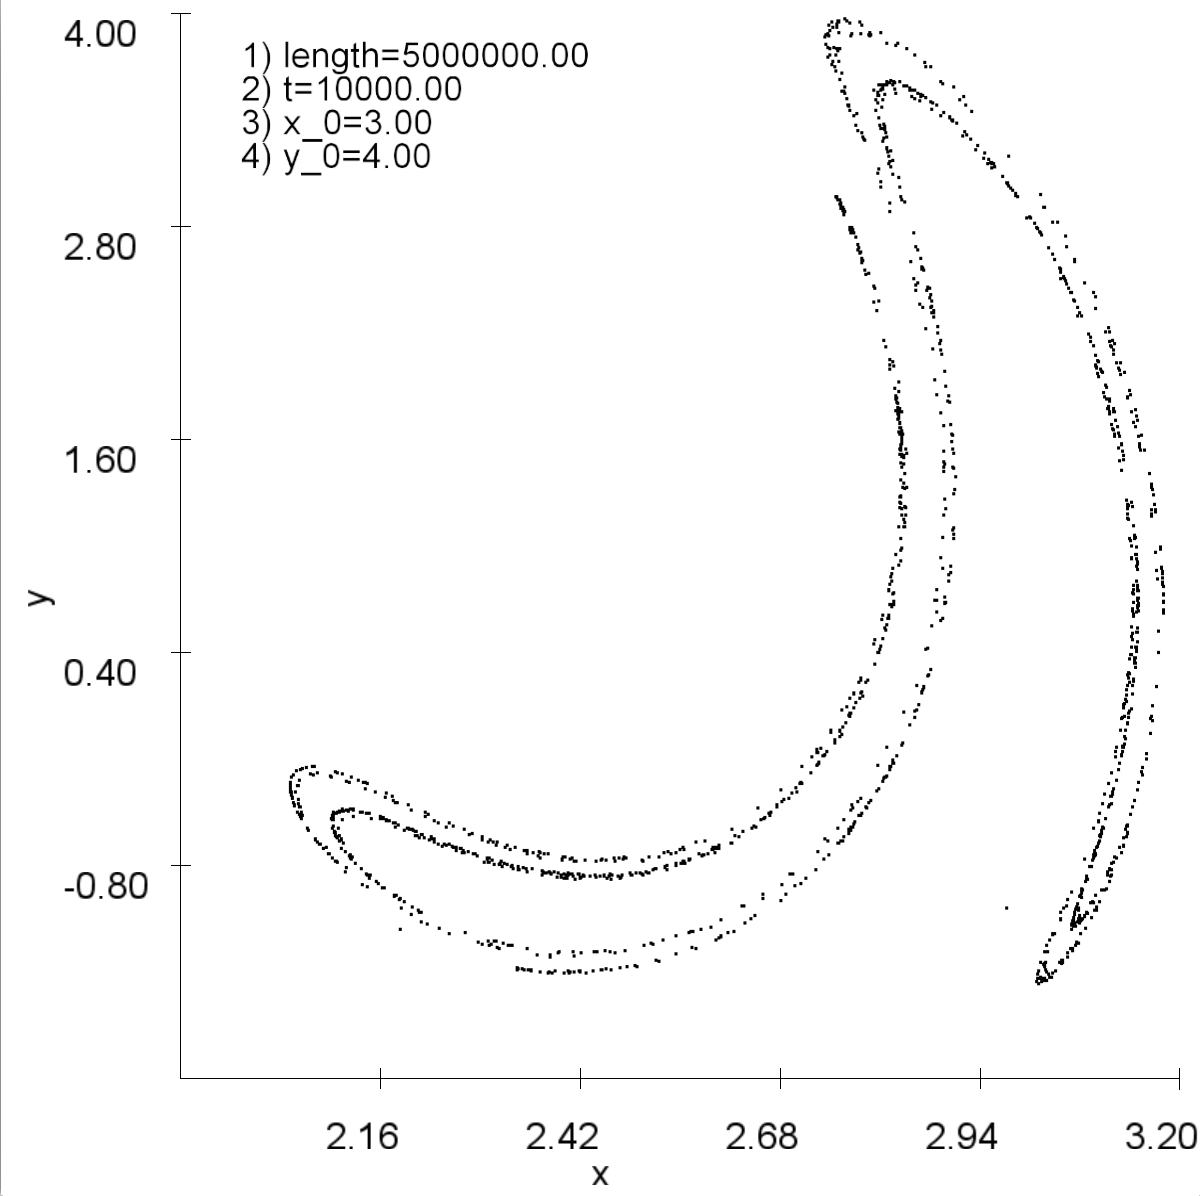
\includegraphics[scale=0.20]{poincare-772}
	\caption{Poincaré-Schnitt des Duffing Oszillators für $\epsilon=7.72$, $x=3.0$,$ y=4.0$, $\lambda=0.2$, $\beta=1$, $\theta=1$. als Referenz aus dem VORBEREITUNGSHEFT-LITERATUR-S38}
	\label{img:poincare-772}
\end{figure}
\section {LDR-Oszillator}
Im folgenden untersuchen wir einen realen nichtlinearen Schwingkreis. Dieser wurde realisiert indem bei einem LCR-Schwingkreis der Kondensator durch eine Diode ausgetauscht wurde (Abbildung \ref{img:schaltskizze})
\begin{figure}[!htbp]
	\centering
	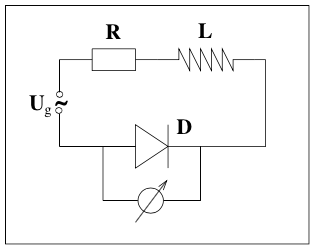
\includegraphics[scale=0.60]{schaltskizze}
	\caption{Schaltskizze für nichtlinearen Schwingkreis. Quelle: Versuchsanleitung, S. 43, Uni Hamburg}
	\label{img:schaltskizze}
\end{figure}

\subsection { Theorie } \label{ssec:theo}
Zunächst lässt sich ein linearer Schwingkreis der aus einem Widerstand, einem Kondensator und einer Spule besteht über die Spannungen an den einzelnen Bauteilen beschreiben
$$V_g=V_c+V_l+V_r \text{ (Kirschoff'sches Gesetz)}$$
Daraus folgt mit $V_g=V_s\cos{\omega t}$ die Differentialgleichung
$$\ddot{Q}L + \dot{Q}R+ \frac{Q}{C} = V_s\cos{\omega t}$$
welche mit dem angetriebenen, gedämpften Oszillator vergleichbar ist. Dabei ist $Q$ die Ladung, $L$ die Induktivität der Spule, $R$ der Widerstand, C die Kapazität des Kondensators $V_s$, die angelegte Spannung und $\omega$ die Frequenz der angelegten Wechselspannung.
\newline
Wird nun der Kondensator durch eine Diode ausgetauscht erhalten wir, wie bei dem Duffing-Oszillator eine Gleichung die nicht mehr analytisch lösbar ist. Während beim linearen Schwingkreis $I=\frac{dQ}{dt}$ gilt lässt sich die Diode als parallel geschalteter Kondensator und Widerstand mit 
\begin{equation}I=I_f(1-\exp(-\frac{V_d}{V_t})) + \frac{dQ}{dt}\end{equation}
beschreiben, wobei $I_f$ und $V_t$ Konstanten sind. Dabei beschreibt der erste Summand den Strom durch den Widerstand und der zweite die Änderung der Ladung aufgrund der Diodenkapazität. 
Dies führt bei einer Kapazität in Durchlassrichtung von $C=C_f\exp(-\frac{V_d}{V_t})$ zu
\begin{equation}\frac{dV_d}{dt}= \frac{I-I_f(1-\exp(-\frac{V_d}{V_t}))}{C_f\exp(-\frac{V_d}{V_t})} \end{equation}
und bei einer Kapazität in Sperrrichtung von $C=C_r(1+\frac{V_d}{\phi})^{-\gamma}$ zu
\begin{equation}
\frac{dV_d}{dt}= \frac{I-I_f(1-\exp(-\frac{V_d}{V_t}))}{C_r(1+\frac{V_d}{\phi})^{\gamma}}
\end{equation}
,wobei $\phi$ und $\gamma$ Konstanten sind.
Außerdem gilt
\begin{equation}\frac{dI}{dt}=\frac{V_s \cos{\theta} - V_d - RI}{L}\end{equation}
\begin{equation}\frac{d\theta}{dt}=\omega\end{equation}
Diese Gleichungen lassen sich numerisch lösen.
\subsection{ Numerische Berechnungen } \label{ssec:num}
Unter Verwendung der Parameter:
\begin{center}
    \begin{tabular}{ | l | l | p{5cm} |}
    \hline
    $R$ & $100\Omega$ & Widerstand \\ \hline
    $L$ & $2367\cdot10^{-6} H$ & Spule \\ \hline
    $C_r$ & $82 pF$ & Konstante proportional zur Kapazität der Diode in Sperrrichtung \\ \hline
    $C_f$ & $56 \cdot10^{-6}  pF$ & Konstante proportional zur Kapazität der Diode in Durchlassrichtung \\ \hline
    $I_f$ & $2,8pA$ & Konstante proportional zum Strom  \\ \hline
    $\gamma$ & $0,44$ & Konstante \\ \hline
    $\phi$ & $0,6V$ & Konstante \\ \hline
    $V_t$ & $34mV$ & Konstante \\
    \hline
    \end{tabular}
\end{center}

haben wir für unterschiedliche Anregungsspannungen $V_s$ numerisch die Gleichungen aus  \ref{ssec:theo} gelöst. Dabei sind wir davon ausgegangen, dass für $V_d > -0.6V$ die Diode sperrt.
\newline
Um sinnvolle Lösungen zu erhalten muss für die Schrittweite $h \geq 10^{-8}$ gelten. Diese oszillierenden Lösungen für den Strom und die Spannung über der Diode sind in Abbildung \ref{fig:ldr-oszi} dargestellt. Strom und Spannung oszillieren mit gleicher Phase und Pendeln sich nach gewisser Zeit unabhängig von den Anfangsbedingungen ein.
\begin{figure}[!htbp]
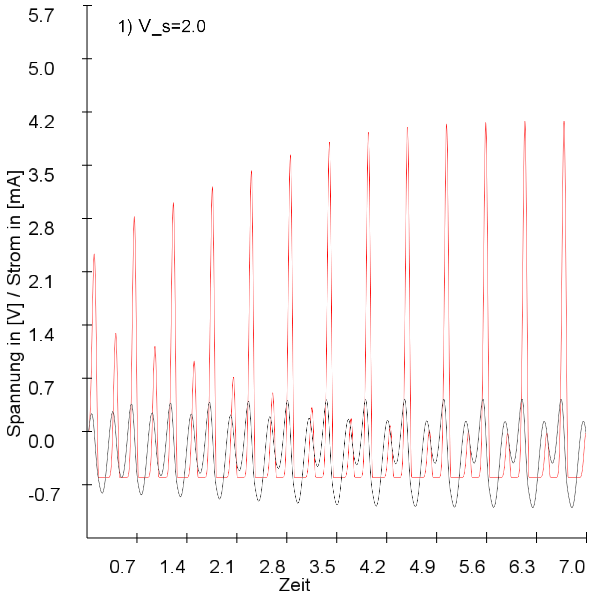
\includegraphics[scale=0.7]{runge-oszillation-100k-2V}
\caption{Oszillation von Strom (schwarz) und Spannung (rot) bei $V_s=2V$ mit Runge-Kutta-Verfahren 4ter Ordnung}. 
\label{fig:ldr-oszi}
\end{figure}
\subsubsection{Phasenraumdiagramme}
Bei einer Anregungsspannung $V_s < 0.001V$ zeigt sich das Verhalten im Grenzfall des gedämpften Oszillators (siehe Abbildung \ref{fig:ldr-0001}).
\begin{figure}[!htbp]
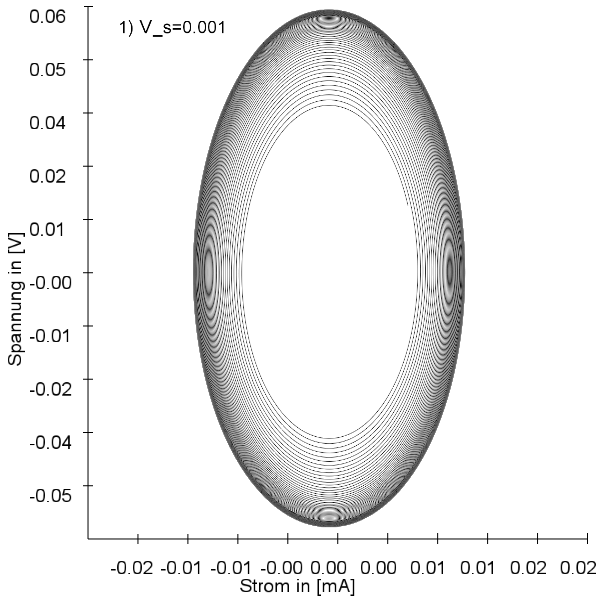
\includegraphics[scale=0.28]{schwing-runge-nach50k-weitere200k-10-9}
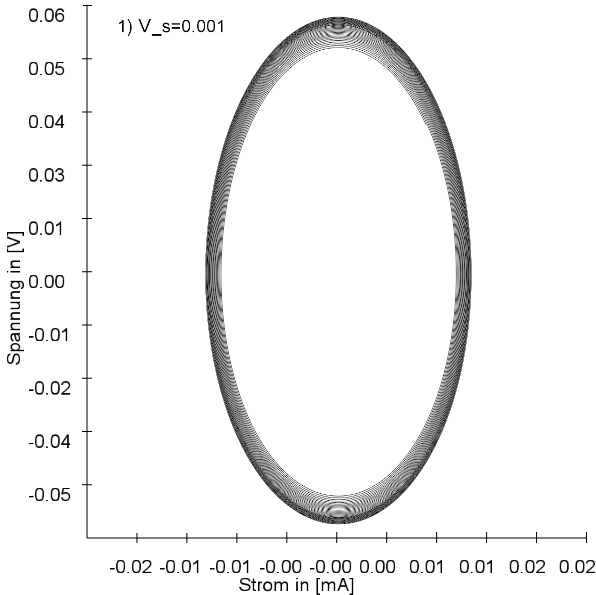
\includegraphics[scale=0.28]{schwing-runge-nach100k-weitere200k-10-9}
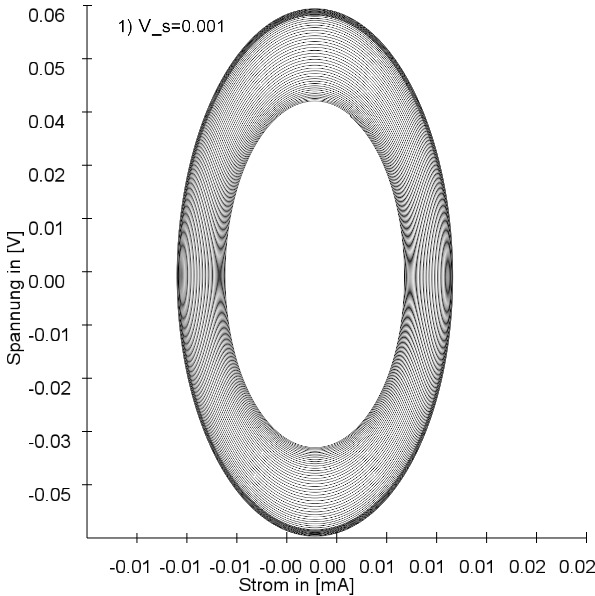
\includegraphics[scale=0.28]{schwing-runge-nach200k-weitere200k-10-9}
\caption{Phasenraumdiagramm mit Runge-Kutta 4ter Ordnung für $V_s=0.001V$ mit $2\cdot10^5$ Zeitschritte bei einer Schrittweite von $h=10^{-9}$. Links: Nach $5\cdot10^4$ Zeitschritten Einschwingzeit, Mitte: Nach $10^2$ Zeitschritten Einschwingzeit. Rechts: Nach $2\cdot10^5$ Zeitschritten Einschwingzeit}. 
\label{fig:ldr-0001}
\end{figure}
Eindeutige Attraktoren erhalten wir bei Spannungen ab $V_s=1V$ (Abbildung \ref{fig:ldr-0002}). Dabei ist bei $V_s=1V$ (links) die Trajektorie wohl definiert, während bei $V_s=1.2V$ (mitte) sie sich langsam aufspaltet und bei $V_s=1.42V$ (rechts) auf 2 Pfaden durch den Phasenraum verläuft.
\begin{figure}[!htbp]
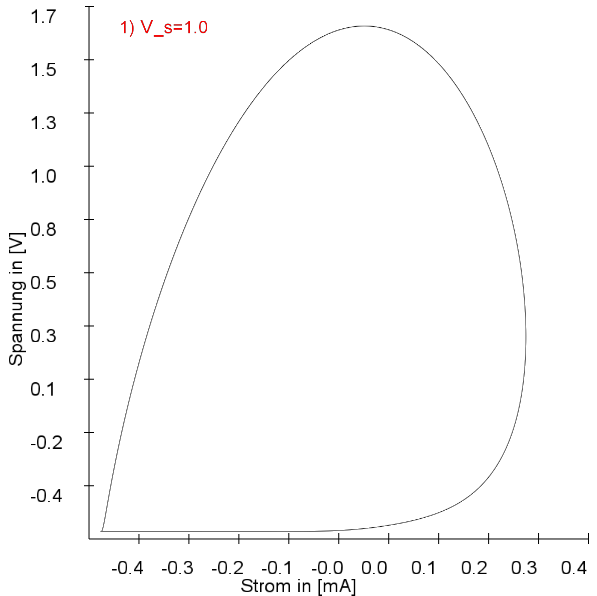
\includegraphics[scale=0.28]{schwing-runge-nach300k-weitere20k-10-9-1V}
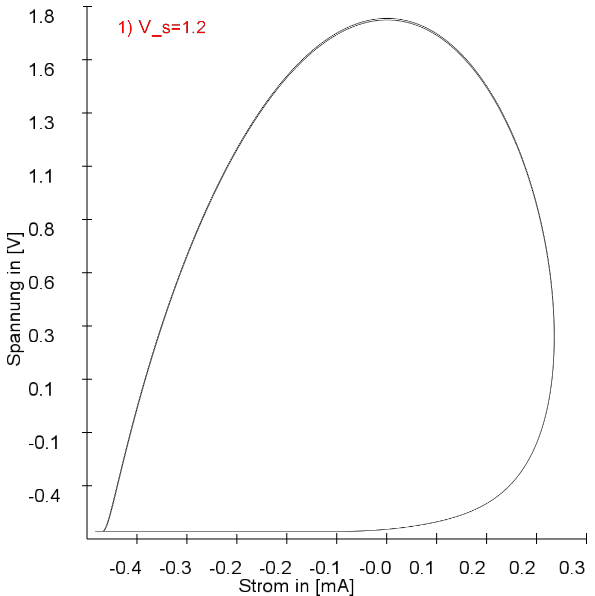
\includegraphics[scale=0.28]{schwing-runge-nach300k-weitere20k-10-9-1,2V}
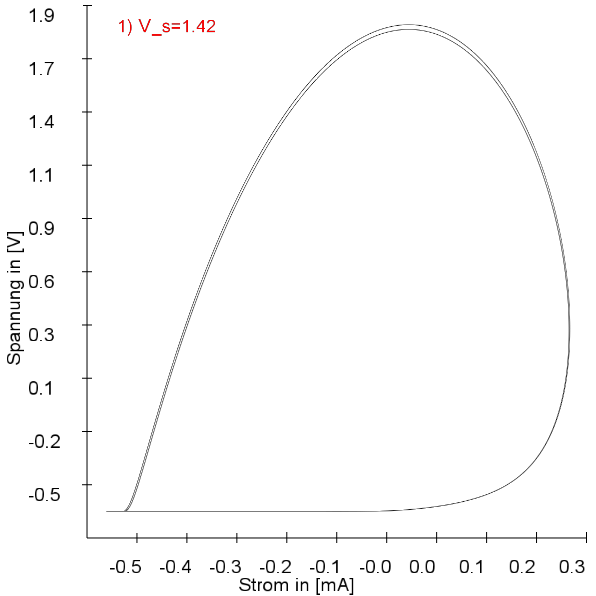
\includegraphics[scale=0.28]{schwing-runge-nach300k-weitere20k-10-9-1,42V}
\caption{Phasenraumdiagramm mit Runge-Kutta 4ter Ordnung für $2\cdot10^4$ Zeitschritte nach einer Einschwingzeit von  $3\cdot10^5$ Zeitschritten und einer Schrittweite von $h=10^{-9}$. Links: $V_s=1V$, Mitte: $V_s=1.2V$. Rechts: $V_s=1.42V$}. 
\label{fig:ldr-0002}
\end{figure}
Je höher $V_s$ wird, desto stärker gehen die Trajektorien auseinander bis sie bei ca. $V_s=20V$ ein Maximum erreichen (Abbildung \ref{fig:ldr-0003} links) und anschließend wieder zusammen gehen und chaotisches verhalten zeigen (Abbildung \ref{fig:ldr-0003} mitte und rechts).
\begin{figure}[!htbp]
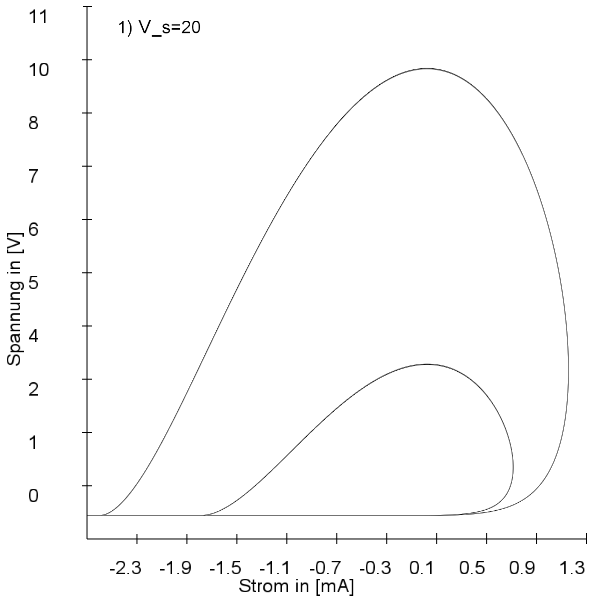
\includegraphics[scale=0.28]{schwing-runge-nach300k-weitere20k-10-9-20V}
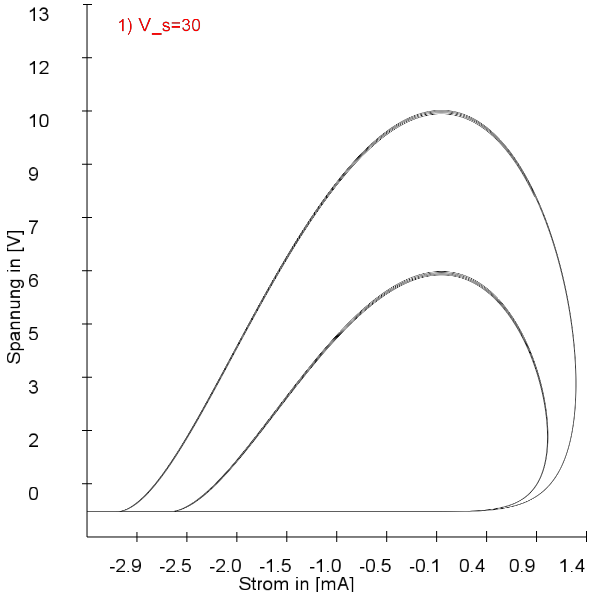
\includegraphics[scale=0.28]{schwing-runge-nach300k-weitere20k-10-9-30V}
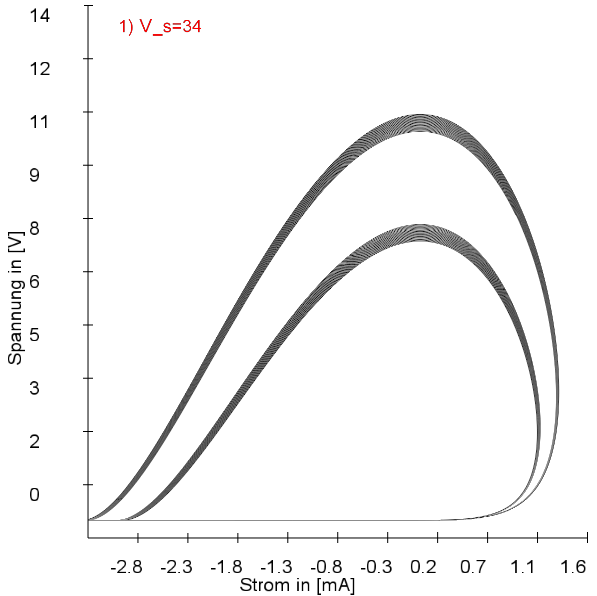
\includegraphics[scale=0.28]{schwing-runge-nach300k-weitere120k-10-9-34V}
\caption{Phasenraumdiagramm mit Runge-Kutta 4ter Ordnung nach einer Einschwingzeit von  $3\cdot10^5$ Zeitschritten und einer Schrittweite von $h=10^{-9}$. Links: $V_s=20V$ für $2\cdot10^4$ Zeitschritte, Mitte: $V_s=30V$ für $2\cdot10^4$ Zeitschritte. Rechts: $V_s=34V$ für $1.2\cdot10^5$ Zeitschritte}. 
\label{fig:ldr-0003}
\end{figure}
\newline
Nach Änderung des Zeitschrittes $h$ auf $h=10^{-8}$ haben wir sehr unterschiedliche Beobachtungen gemacht. Beispielsweise erhalten wir bei $V_s=9.1300024986267072V$ einen eindeutigen Attraktor (Abbildung \ref{fig:ldr-0004} links) und Chaos bei einer einem Wert $10^{-15}V$ größer (rechts).
\begin{figure}[!htbp]
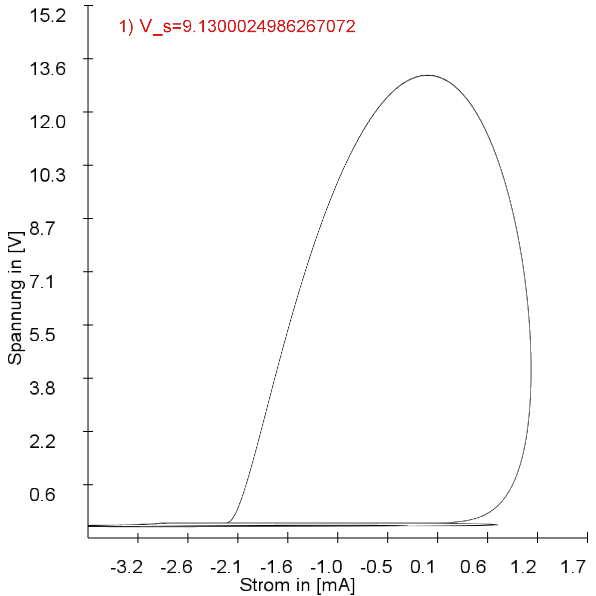
\includegraphics[scale=0.42]{schwing-runge-nach300k-weitere50k-10-8-searching-chaos1}
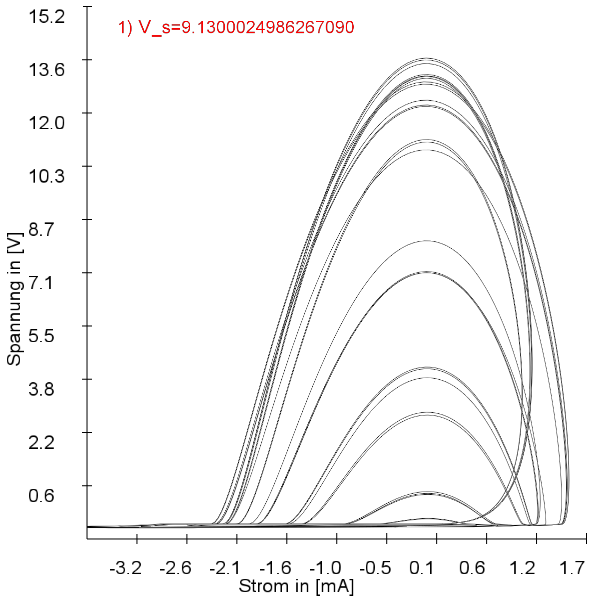
\includegraphics[scale=0.42]{schwing-runge-nach300k-weitere50k-10-8-finding-chaos1}
\caption{Phasenraumdiagramm mit Runge-Kutta 4ter Ordnung nach einer Einschwingzeit von  $3\cdot10^5$ Zeitschritten für weitere $5\cdot10^4$ Zeitschritte bei einer Schrittweite von $h=10^{-8}$. Links: Wohldefinierter Attraktor. Rechts: Chaos}. 
\label{fig:ldr-0004}
\end{figure}
Unter Verwendung des Euler-Cauchy-Verfahrens beobachten wir teilweise ein anderes Verhalten. So können wir im Bereich von $V_s=3V$ bis $V_s=4.7V$ mehrere Periodenverdopplungen beobachten (Abbildung \ref{fig:ldr-0005} und \ref{fig:ldr-0006}) bis hin zum Chaos.
\begin{figure}[!htbp]
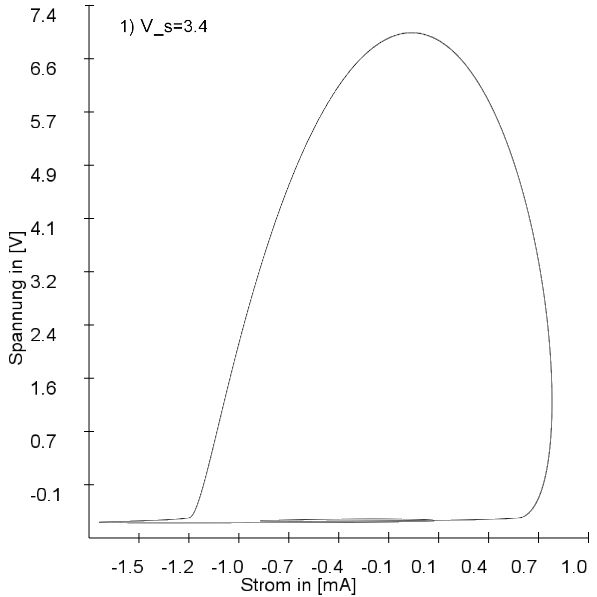
\includegraphics[scale=0.42]{schwing-euler-nach2500k-weitere100k-3,4V}
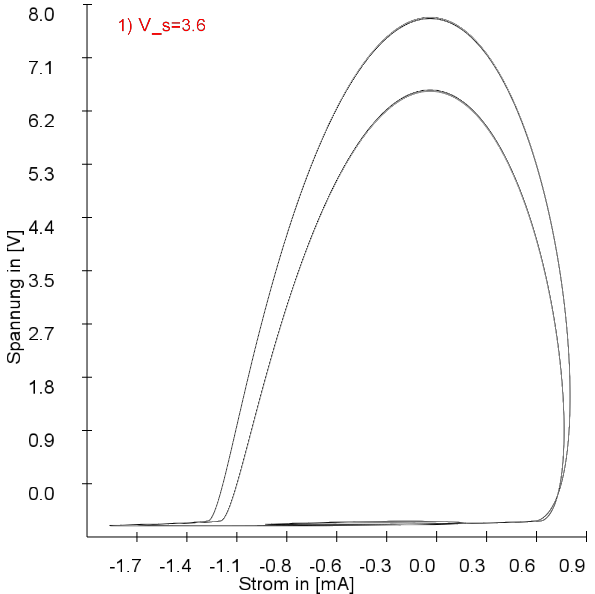
\includegraphics[scale=0.42]{schwing-euler-nach2500k-weitere100k-3,6V}
\caption{Phasenraumdiagramm mit Euler-Cauchy-Verfahren nach Einschwingzeit von $2.5\cdot10^6$ Zeitschritten für weitere $10^5$ Zeitschritte. Links: $V_s=3.4V$, Rechts: $V_s=3.6V$}. 
\label{fig:ldr-0005}
\end{figure}
\begin{figure}[!htbp]
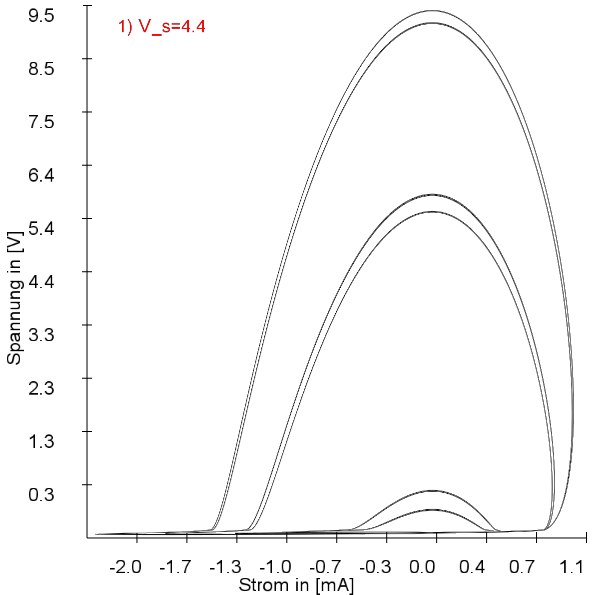
\includegraphics[scale=0.42]{schwing-euler-nach2500k-weitere100k-4,4V}
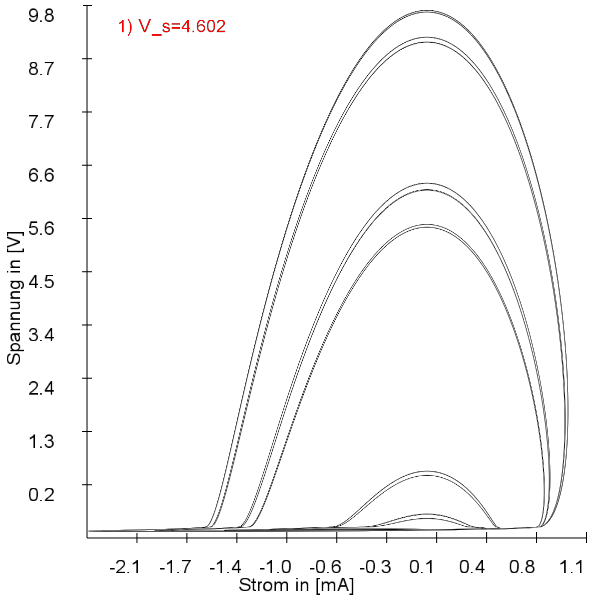
\includegraphics[scale=0.42]{schwing-euler-nach2500k-weitere100k-4,602V}
\caption{Phasenraumdiagramm mit Euler-Cauchy-Verfahren nach Einschwingzeit von $2.5\cdot10^6$ Zeitschritten für weitere $10^5$ Zeitschritte. Links: $V_s=4.4V$, Rechts: $V_s=4.602V$}. 
\label{fig:ldr-0006}
\end{figure}

\subsubsection{Poincaré-Schnitt}
Bei der Betrachtung des Poincaré-Schnittes fällt auf, dass bei wohldefinierten Attraktoren die Phasenraumtrajektorie immer bei ähnlichen Spannungen durch die $\theta=0$ Ebene verläuft (vgl. Abbildung \ref{fig:ldr-poin1}).
\begin{figure}[!htbp]
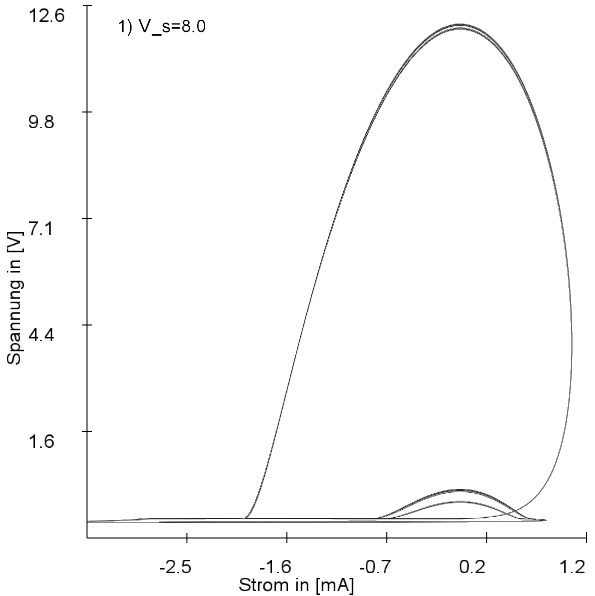
\includegraphics[scale=0.4]{schwing-500k-nach-10k-8V-phase}
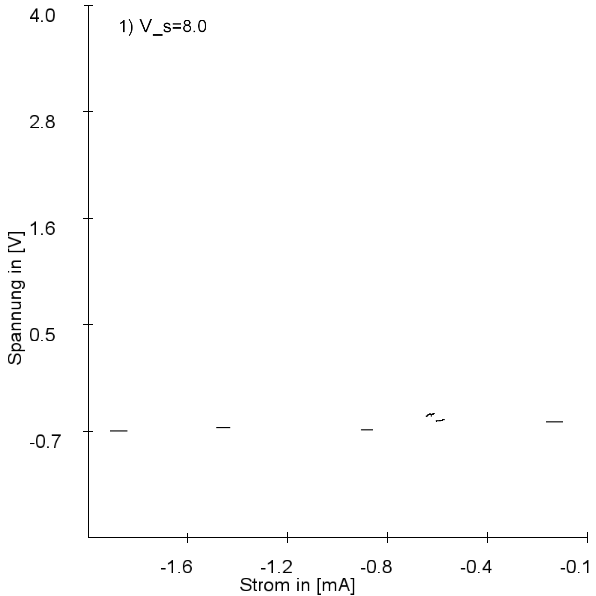
\includegraphics[scale=0.4]{schwing-500k-nach-10k-8V-poin}
\caption{$5\cdot10^5$ Zeitschritte nach einer Einschwingzeit von $\cdot10^4$ Zeitschritten bei $V_s=8V$. Links: Phasenraumdiagramm. Rechts: Poincaré-Schnitt durch $\theta=0$ Ebene}
\label{fig:ldr-poin1}
\end{figure}
 Im chaotischen Fall weißt der Poincaré-Schnitt weitere Punkte bei unterschiedlichen Spannungen auf (vgl. Abbildung \ref{fig:ldr-poin2}).
\begin{figure}[!htbp]
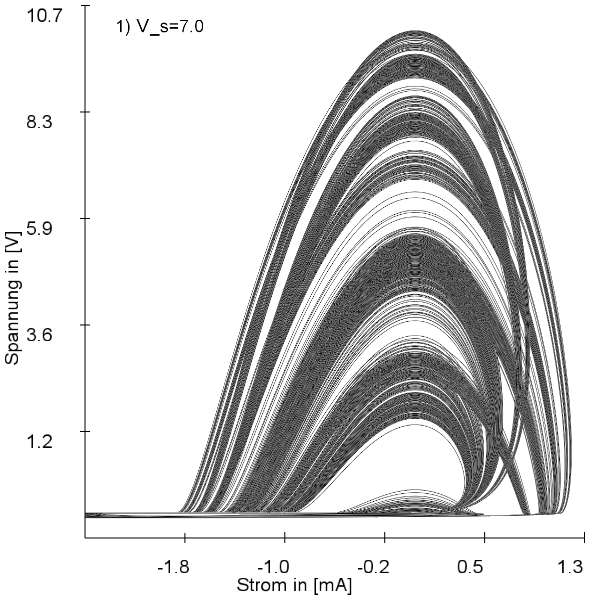
\includegraphics[scale=0.4]{schwing-500k-nach-10k-7V-phase}
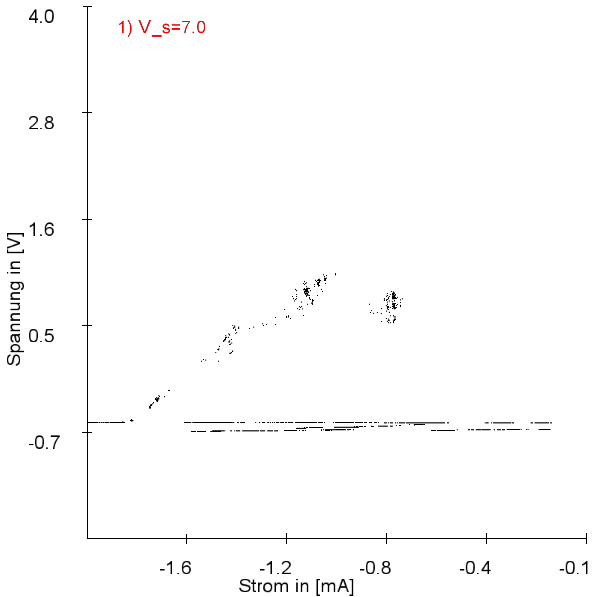
\includegraphics[scale=0.4]{schwing-500k-nach-10k-7V-poin}
\caption{$5\cdot10^5$ Zeitschritte nach einer Einschwingzeit von $\cdot10^4$ Zeitschritten bei $V_s=7V$. Links: Phasenraumdiagramm. Rechts: Poincaré-Schnitt durch $\theta=0$ Ebene}
\label{fig:ldr-poin2}
\end{figure}
Anmerkung: Bei der numerischen Berechnung  kommt es immer wieder vor, dass bei ganz bestimmten $V_s$ der Open-GL Buffer auf der Grafikkarte überläuft.
\subsubsection{Bifurkationsdiagramm-Diagramm}
Um den Bereich von Chaos und Ordnung zu visualisieren, haben wir im folgenden separat für Strom und Spannung das Bifurkationsdiagramm geplottet. Dabei ist der variierende Parameter die Eingangsspannung $V_s$.
\begin{figure}[!htbp]
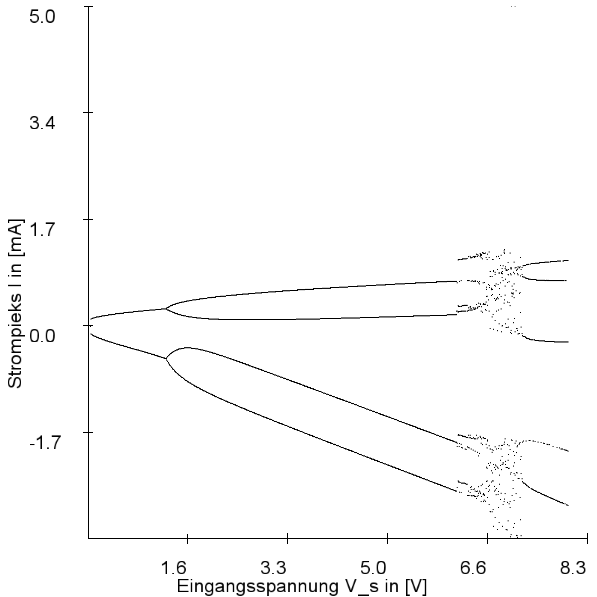
\includegraphics[scale=0.4]{schwing-bifurc-von-0-8-in-0,01schritten-400k-strom}
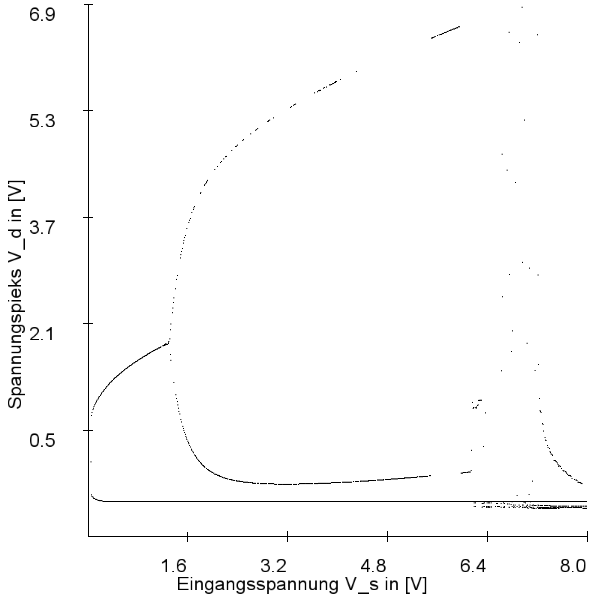
\includegraphics[scale=0.4]{schwing-bifurc-von-0-8-in-0,01schritten-400k-spannung}
\caption{Bifurkationsdiagramm mit $4\cdot10^5$ Iterationen pro $V_s$. Von $V_s=0$ bis $V_s=8$ in $0.01$ Schritten. Links: Strom. Rechts: Spannung}
\label{fig:ldr-bifurc}
\end{figure}
Bei $V_s\approx1.4$ beobachten wir sowohl beim Strom als auch bei der Spannung eine Periodenverdopplung.Dies passt mit unserer Beobachtung des Attraktors bei $V_s=1.42$ (Abbildung \ref{fig:ldr-0002} rechts) zusammen. Auch das Chaotische Verhalten bei $V_s=7$ (Abbildung fig:ldr-poin2 links) finden wir im Bifurkationsdiagramm wieder.

\subsection{ Versuchsaufbau}
Für die Messung an einem realen LDR-Schwingkreis haben wir zunächst einen Messaufbau wie in Abbildung \ref{fig:ldr-aufbau1} (links) verwendet. Über die Eingänge A und B des Oszilloskop konnten wir Strom und Spannung über der Diode einzeln und als Phasendiagram darstellen. Ferner haben wir einen Gate-Delay Generator verwendet der \ref{fig:ldr-aufbau1} (rechts) zusehen ist. TODO: Abbildungen noch nicht korrekt.
\begin{figure}[!htbp]
\includegraphics[scale=0.6]{aufbau1}
\includegraphics[scale=0.5]{aufbau2}
\caption{Messaufbau zur Visualisierung des LDR-Schwingkreises. Oszilloskop links zur Überprüfung der Eingangsspannung und Frequenz. Links: Strom und Spannung über der Diode werden dargestellt auf Oszilloskop über Eingänge A und B. Rechts: Gate-Delay Einheit verzögert Signal in Abhängigkeit der jetzt variierenden Eingangsspannung $V_s$ zur Darstellung des Stroms bzw. der Spannung in Abhängigkeit von $V_s$ }
\label{fig:ldr-aufbau1}
\end{figure}
Die Parameter des Schwingkreises unterscheiden sich von den Paramtern, die bei der numerischen Berechnung verwendet wurden. So hatten wir eine gesamt Induktivität von $L\approx370\cdot10^{-6}H$ was bei einer Resonanzfrequenz von $w\approx800kHz$ zu $C_r\approx4.2\cdot10^{-9}F$ führt.
\subsection { Versuchsdurchführung }
\subsubsection { Oszillation und Phasenraumdiagram }
Zunächst haben wir bei bei einer Eingangsspannung von $V_s=0.128V$ die Resonanzfrequenz über die Betrachtung des Phasenraumdiagramms auf $\omega=800kHz$ bestimmt. 
Der aufgebaute Schaltkreis hatte nicht die selbe Konfiguration wie unsere numerischen Modelle, dennoch erhalten wir einen sehr ähnlichen Verlauf. In Abbildung \ref{fig:ldr-real1} sind die Oszillationen von Strom und Spannung (links) und das entsprechende Phasenraumdiagram dargestellt (rechts) welches dem numerischen Ergebniss in \ref{fig:ldr-0005} (links) sehr ähnlich sieht. 
\begin{figure}[!htbp]
\centering
\includegraphics[scale=0.1]{800khz-5V-oszi}
\includegraphics[scale=0.11]{800khz-5V-phase}
\caption{Eingangsspannung $V_s=5V$ und Resonanzfrequenz von $\omega=800kHz$. Links: Zeitlicher Verlauf von Spannung (oben) und Strom (unten). Rechts: Phasenraumdiagram}
\label{fig:ldr-real1}
\end{figure}

\begin{figure}[!htbp]
\centering
\includegraphics[scale=0.05]{800khz-134V-phase}
\includegraphics[scale=0.055]{800khz-112V-phase}
\includegraphics[scale=0.06]{800khz-29,6V-phase-chaos}
\caption{Eingangsspannung $V_s=5V$ und Resonanzfrequenz von $\omega=800kHz$. Links: Zeitlicher Verlauf von Spannung (oben) und Strom (unten). Rechts: Phasenraumdiagram}
\label{fig:ldr-real2}
\end{figure}
\subsection { Bifurkationsdiagramm }
Beim erzeugen des Bifurkationsdiagrammes haben wir einen anderen Schaltkreis verwendet, dessen Resonanzfrequenz wir auf $\omega=325kHz$ bestimmt haben. Der Versuchsaufbau wurde nun mit einer Gate-Delay Einheit aufgebaut (Abbildung \label{fig:ldr-aufbau1}). Wir modelierten über den Aux-Out des Funktionsgenerator eine Sägezahnspannung welche später den Definitionsbereich des Kontrollparameters $V_s$ darstellt. 
Zunächst ist dies nicht gelungen. Mit Hilfe des digitalen Oszilloskopes konnten wir dann aber den Verlauf so modelieren, dass  $V_s=0V...V_s=V_{Ausgang}$ linear perdiodisch durchlaufen wird. 
Wir stellten fest, dass das Bifurkationsdiagramm am besten am Oszilloskop zu sehen war, wenn wir den Definitionsbereich von oben nach unten ($V_s=V_{Ausgang}...V_s=0V$) eingestellt haben (Abbildung \ref{fig:ldr-modellierung}). In dieser Einstellung gab es zwar noch Artefakte von der Ungenauigkeit des Funktionsgenerators (Abbildung \ref{fig:ldr-modellierung} rechts) aber die Bifurkationspunkte waren nun präziser. Wir erzeugten das Bifurkationsdiagramm zusätzlich mit einer Dreieckspannung. Wie zu erwarten ergab sich so eine Überlageung aus den beiden Sägezahnspannungen. 
\begin{figure}[!htbp]
\centering
\includegraphics[scale=0.12]{bif-ldr/dreieck_1}
\includegraphics[scale=0.12]{bif-ldr/dreieck_2}
\includegraphics[scale=0.12]{bif-ldr/dreieck_3}
\caption{Bifurkationsdiagramme mit verschieden Modulationen des Kontrollparameters $V_s$: Links Sägezahnspannung $V_s=0V...V_s=V_{Ausgang}$, mitte: Dreiecksspannung, rechts: Sägezahnspannung $V_s=V_{Ausgang}...V_s=0V$}
\label{fig:ldr-modellierung}
\end{figure}

Wir fragten uns, wieso es zu einer Spitze im oberen Ast nach der ersten Bifuraktion kommt. Dabei zeigte sich, dass die Frequenz nicht genau auf  $\omega=325kHz$ eingestellt war. Als wir dies korrigierten erhielten wir ein glatteres Bifurkationsdiagramm (Abbildung N)

\begin{figure}[!htbp]
\centering
\includegraphics[scale=0.18]{bif-ldr/bifurc-bad}
\includegraphics[scale=0.18]{bif-ldr/bifurc-good}
\caption{Eingangsspannung $V_s=5V$ und Resonanzfrequenz von $\omega=800kHz$. Links: Zeitlicher Verlauf von Spannung (oben) und Strom (unten). Rechts: Phasenraumdiagram}
\label{fig:ldr-bifurc}
\end{figure}
\subsection { Vermessung der Bifurkationspunkte }
Zuletzt haben wir noch die Bifurkationspunkte vermessen. Dazu haben wir die Amplitude der Sägezahnspannung minimiert, so dass $V_s=V_{Ausgang}$ konstant war. Bei geringer Spannung wurde auf dem Oszilloskop nur ein Punkt abgebildet. Beim durchlaufen der Spannung entstanden so sprungartig zwei Punkte und schließlich 4 Punkte. Die jeweiligen $V_{Bifurkation, i}$ konnten wir somit als Bifurkationspunkte identifizieren: 
$$V_{Bifurkations, 1}=6.6V \pm 0.2V$$
$$V_{Bifurkations, 2}=13.6V \pm 0.2V$$

In Abbildung \ref{fig:ldr-bifurc-zoo} haben wir noch ein mal mit der Sägezahnspannung die Bifurkationspunkte vergrößert aufgenommen. Es gelang uns nicht den Bifurkationspunkt $_{Bifurkations, 3}$ zu bestimmen weshalb wir die Feigenbaumkonstante nicht aus dem Experiment ableiten konnten.

\begin{figure}[!htbp]
\centering
\includegraphics[scale=0.18]{bif-ldr/bifurc-zoom}
\includegraphics[scale=0.18]{bif-ldr/bifurc-zoom2}
\caption{Vergrößerung der ersten beiden Bifurkationspunkte.}
\label{fig:ldr-bifurc-zoom}
\end{figure}


\subsection { Zusammenfassung }

\section{ Literatur }
\nocite{*}
\printbibliography
\begin{itemize} 
\item Nichtlineare Dynamik und Chaos - Physikalisches Praktikum für Fortgeschrittene Universität Hamburg
\end{itemize}

\section{Appendix}
\subsection {Runge-Kutta 4ter Ordnung in 3 Dimensionen}
Hängt $f$ von mehr als nur x und t ab, so lassen sich weitere Parameter ebenfalls mit der selben Idee variieren.
Gegeben seien folgende Differentialgleichungen:
$$\frac{dx}{dt}=f(x,y,t)$$
$$\frac{dy}{dt}=g(x,y,t)$$
Dann definieren wir im Sinne des Runge-Kutta Verfahrens:
$$k_1 = hf(x_n,y_n,t)$$
$$l_1 = hg(x_n,y_n,t)$$
$$k_2 = hf(x_n+h\frac{k_1}{2},y_n+h\frac{l_1}{2},t+\frac{h}{2})$$
$$l_2 = hg(x_n+h\frac{k_1}{2},y_n+h\frac{l_1}{2},t+\frac{h}{2})$$
$$k_3 = hf(x_n+h\frac{k_2}{2},y_n+h\frac{l_2}{2},t+\frac{h}{2})$$
$$l_3 = hg(x_n+h\frac{k_2}{2},y_n+h\frac{l_2}{2},t+\frac{h}{2})$$
$$k_4 = hf(x_n+hk_3,y_n+hl_3,t+h)$$
$$l_4 = hg(x_n+hk_3,y_n+hl_3,t+h)$$
Und schließlich:
$$y_{n+1} = y_n + \frac{k_1 + 2k_2 + 2k_3 + k_4}{6}$$
$$x_{n+1} = x_n + \frac{l_1 + 2l_2 + 2l_3 + l_4}{6}$$




\end{document}







